\documentclass[letterpaper, 11pt]{article}
\usepackage{comment} % enables the use of multi-line comments (\ifx \fi) 
\usepackage{fullpage} % changes the margin
\usepackage{fancyhdr} % for footer
\usepackage[UKenglish]{isodate}% http://ctan.org/pkg/isodate for date format
\usepackage{float}%force tables/figs into certain placement
\usepackage{changepage}%for dichotomous key
\usepackage{graphicx}%for figures
\usepackage{subcaption}%for figures
\usepackage{hyperref}%for links
\usepackage[font=small,labelfont=bf]{caption}%for captions
\usepackage[letterpaper,margin=1in]{geometry}
\usepackage{natbib}	%for bibliography
\usepackage{placeins}%prevent images from floating into inappropriate sections

\def\labelitemi{--}

\pagestyle{fancy}
\renewcommand{\headrulewidth}{0pt}

\lhead{}
\chead{}
\rhead{}
\lfoot{ENT 432 (Fall 2015) - Penn State}
\cfoot{}
\rfoot{\thepage}
\renewcommand{\footrulewidth}{0.4pt}
\title{Unit 9 - Acercaria}
\author{}

\begin{document}
\cleanlookdateon %removed ordinal date
\maketitle
\thispagestyle{fancy}
\section*{Introduction}
Here we begin looking at taxa classified in \textbf{Acercaria}, a taxon characterized in part by their stylate laciniae. These three orders, Psocodea, Thysanoptera, and Hemiptera, may comprise a monophyletic lineage that is sister to Holometabola (the taxon with truly larval immature stages). Alternatively, based on genome-scale molecular data \citep{Misof763}, these taxa are related as ((Thysanoptera, Hemiptera),(Psocodea, Holometabola)). Acercaria share the following characteristics \citep{beutel2013insect}; do they represent synapomorphies?

\begin{itemize}
\item legs with $\le$3 tarsomeres
\item cerci absent 
\item labial palps relatively small or absent 
\item maxilla modified into stylet (maxillary laciniae are separated from the rest of the maxilla and are stylet-like)
\item postclypeus relatively large, accommodates cibarial dilator muscles for sucking
\item many species with inactive stage prior to adult
\end{itemize}

\section*{Materials}

\begin{itemize}
\item specimens (provided)
\item fine forceps, probes (provided)
\item sorting tray, watch glasses, gloves, safety glasses, glycerine, ethanol (provided)
\item pencil/paper for sketches
\end{itemize}

\section*{Safety}
We will be working with sharp tools and insects on pins. Wear your personal protective gear at all times. Specimens are to be returned to their vials after lab, and glycerine and ethanol will be collected for proper disposal or reuse.

\section*{Methods}
Working with a partner, organize your space, specimens, tools, and microscope. Use your probe and forceps to manipulate the specimen. In this lab, however, we will not be dissecting specimens (unless otherwise noted). You can start anywhere in the handout.

\section{Psocodea (lice)}
This lineage is comprised of three infraorders; we cover only two. The previously recognized orders are not monophyletic. Synapomorphies of Psocodea include: Specialized water vapor uptake system (sitophore), which we won't see in lab; autotomic antennae (look for line of weakness proximally); molecular data.\\

\subsection{Psocomorpha (bark lice)}
\noindent{}\textit{Diagnostic characters:} Head usually with rounded vertex; antenna with 13 antennomeres; flagellomeres never annulated; labial palpus not subdivided; fore wing with nodus and thickened pterostigma (Figure \ref{fig:psocidwing}); CuP ending together with A1 at wing margin; tarsus subdivided into 2--3 tarsomeres.\\

\noindent{}There are 24 families classified in Psocomorpha. In lab we will look at only one: \textbf{Psocidae} (Figure \ref{fig:psocid}).

\begin{figure}[ht!]
 \centering
 \begin{subfigure}[ht!]{0.45\textwidth}
  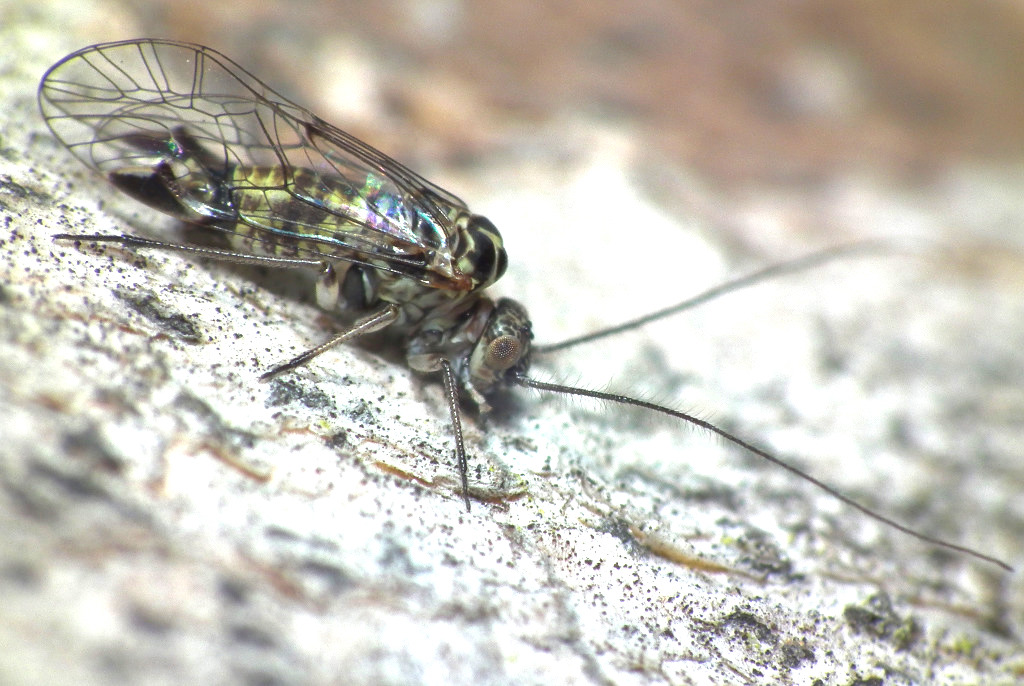
\includegraphics[width=\textwidth]{PsocidHabitus}
  \caption{Lateral habitus. Photo (CC BY 2.0) by James Niland \url{https://goo.gl/jr0D5W}}
  \label{fig:psocid}
 \end{subfigure}
 \qquad
 \begin{subfigure}[ht!]{0.45\textwidth}
  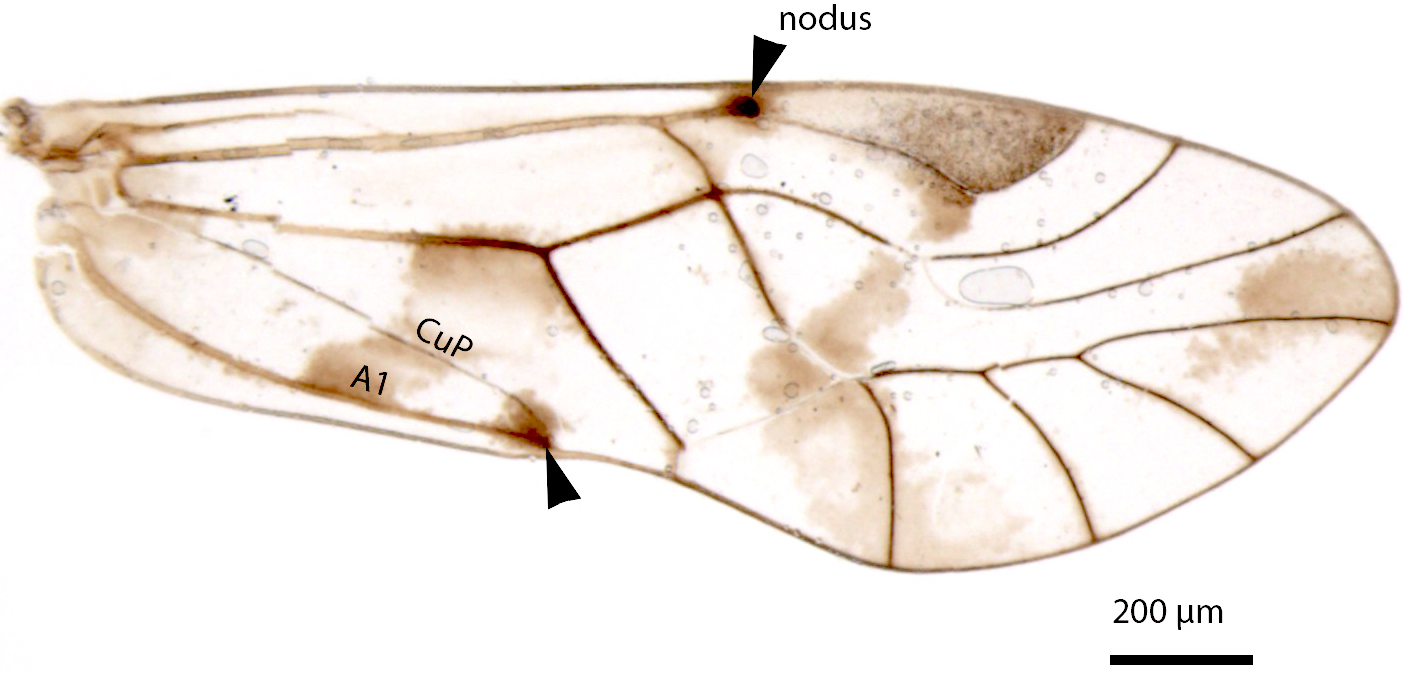
\includegraphics[width=\textwidth]{PsocidWing}
  \caption{Psocomorphan fore wing. Photo (CC BY 2.0) by Istv\'an Mik\'o \url{https://flic.kr/p/z3Svuw}}
  \label{fig:psocidwing}
 \end{subfigure}
 \caption{Psocomorpha}\label{fig:psocids}
\end{figure}

\subsection{Troctomorpha (book and parasitic lice)}
\noindent{}\textit{Diagnostic characters:} Head usually with relatively flat vertex; antenna with 15--17 antennomeres; tarsus subdivided into 2 tarsomeres.\\

\noindent{}There are 9 families classified in Troctomorpha. In lab we will look at four (see below), all of which are wingless and three of which are parasitic. Can you guess which ones, without looking at the common names? What adaptations for parasitism do you see in these taxa?\vspace{4cm}

\subsubsection{Liposcelididae (common book lice)}
\noindent{}\textit{Diagnostic characters:} Body usually yellow-brown in color; head prognathous; antenna relatively long, with 9--15 flagellomeres (Figure \ref{fig:liposcelidid}); tarsus subdivided into 3 tarsomeres; hind femora relatively large; wings absent in most species.\\

\noindent{}\textit{Natural history:} \\

\begin{figure}[ht!]
 \centering
 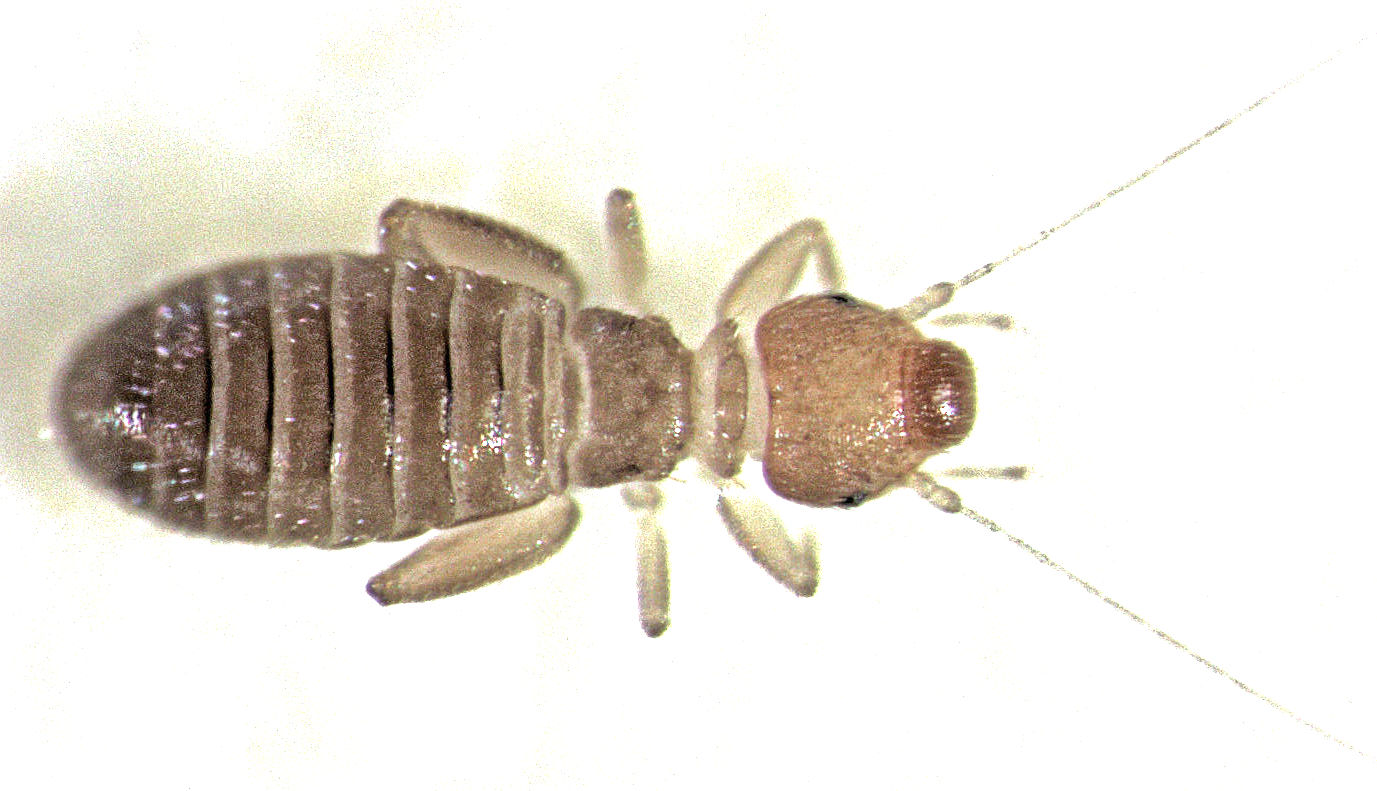
\includegraphics[width=0.5\textwidth]{LiposcelididHabitus}
 \caption{Liposcelididae. Photo (CC0) by S. E. Thorpe \url{https://goo.gl/Gd1yft}}
 \label{fig:liposcelidid}
\end{figure}

\subsubsection{Pediculidae (human head and body lice)}
\noindent{}\textit{Diagnostic characters:} Head usually narrower than prothorax (Figure \ref{fig:pediculid}); fore, mid, and hind legs roughly equal in size; tibial-tarsal complex adapted for grabbing; abdomen longer than width at base.\\

\noindent{}\textit{Natural history:} \\

\begin{figure}[ht!]
 \centering
 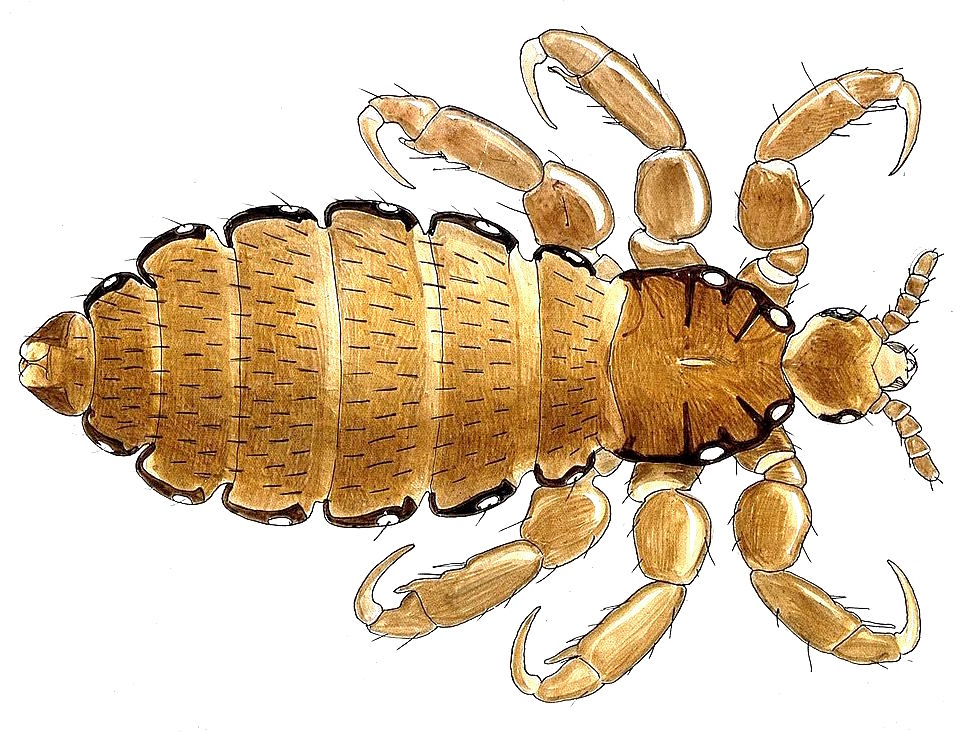
\includegraphics[width=0.4\textwidth]{PediculidHabitus}
 \caption{Pediculidae. Illustration by A. J. E. Terzi, CC BY Wellcome Trust \url{https://goo.gl/GByqFC}}
 \label{fig:pediculid}
\end{figure}

\subsubsection{Phthiridae (human pubic louse, Gorilla louse)}
\noindent{}\textit{Diagnostic characters:} Head narrower than prothorax; mid and hind legs thicker than fore legs; abdomen about as long as its width at base, with prominent lobe-like structures (paratergites) laterally (Figure \ref{fig:phthirid}).\\

\noindent{}\textit{Natural history:} \\

\begin{figure}[ht!]
 \centering
 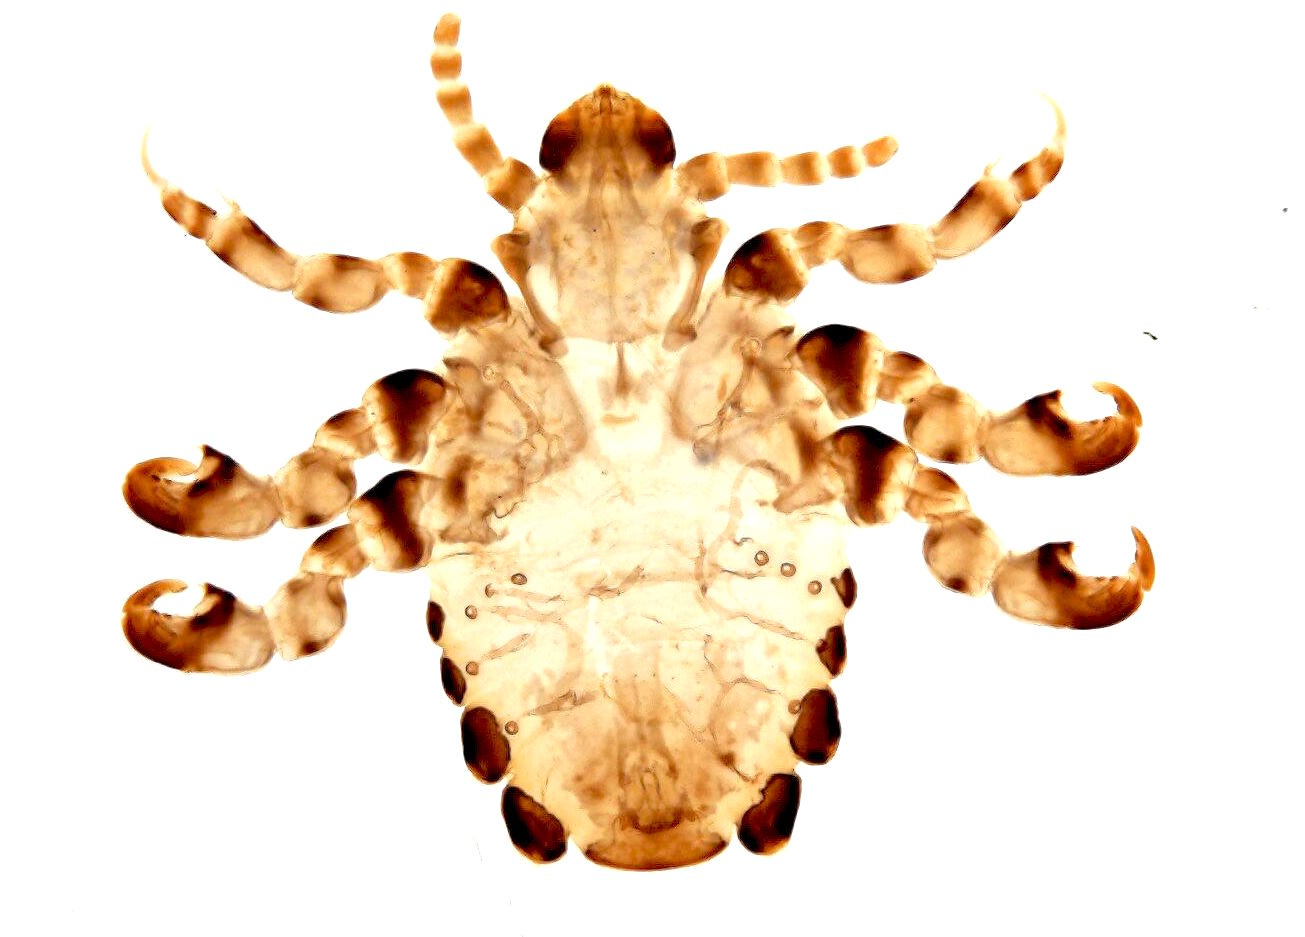
\includegraphics[width=0.45\textwidth]{PhthiridHabitus}
 \caption{Phthiridae. Photo (CC BY 2.0) by Frost Entomological Museum \url{https://flic.kr/p/znDT6y}}
 \label{fig:phthirid}
\end{figure}

\subsubsection{Trichodectidae (mammal chewing lice)}
\noindent{}\textit{Diagnostic characters:} Head as wide as or wider than thorax; mouthparts chewing (mandibulate) (Figure \ref{fig:trichodectid}); antennae filiform, exposed, with 3 antennomeres; maxillary palpi absent. \\

\noindent{}\textit{Natural history:} \\

\begin{figure}[ht!]
 \centering
 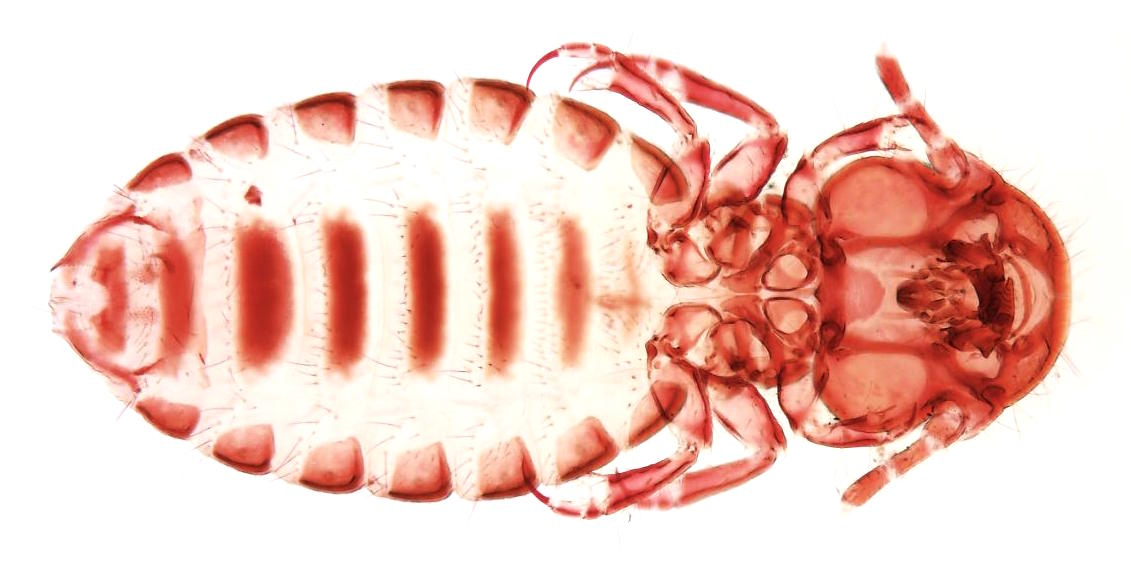
\includegraphics[width=0.45\textwidth]{TrichodectidHabitus}
 \caption{Trichodectidae. Photo (CC BY 2.0) by Emily Sandall \url{https://flic.kr/p/uQweJC}}
 \label{fig:trichodectid}
\end{figure}

\subsection{Trogiomorpha}
\noindent{}\textit{Diagnostic characters:} Antenna with 22--50 antennomeres.\\

\noindent{}There are 7 families classified in Trogiomorpha. We have no specimens in our teaching collection.\\

\section{Thysanoptera (thrips)}
\noindent{}\textit{Diagnostic characters:} Body very small (usually $\sim$2 mm), with opisthognathous head; antenna with 7--9 antennomeres; piercing/sucking, asymmetrical (one mandible present) mouthparts; wings usually narrow with fringe composed of long setae; fore wing similar in size/shape to hind wing; tarsus with 1 or 2 tarsomeres; arolium (apicomedial membraneous area of pretarsus) balloon-shaped, eversible, exceeds tarsal claw apically.\\

\noindent{}Thysanoptera is subdivided into two suborders---Terebrantia (8 families, including Thripidae) and Tubulifera (1 family; Phlaeothripidae). Keep in mind that ``thrips'' is both singular and plural!

\subsection{Terebrantia}
\subsubsection{Thripidae (common thrips)}
\noindent{}\textit{Diagnostic characters:} terminal abdominal segment divided ventrally, cone shaped, with strongly converging lateral margins; ovipositor present (Figure \ref{fig:thripid2}); wing surface with acanthae (microtrichiae, or cuticular protuberances in the wing) and 2 rows of setae. \\

\noindent{}\textit{Natural history:} \\

\begin{figure}[ht!]
 \centering
 \begin{subfigure}[ht!]{0.45\textwidth}
  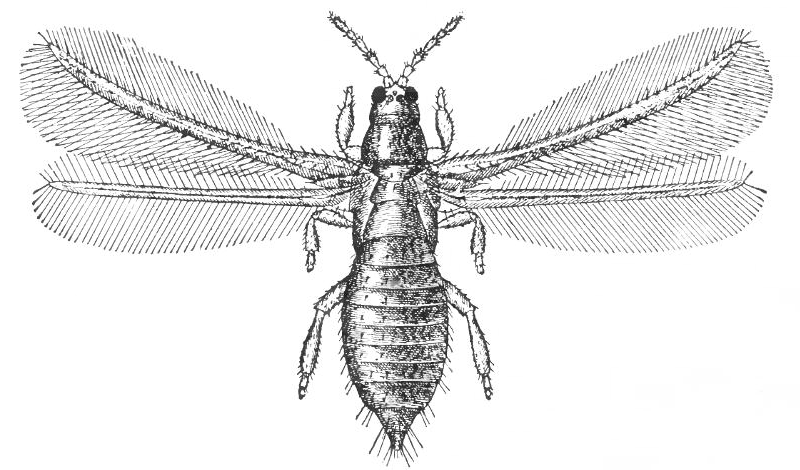
\includegraphics[width=\textwidth]{ThripidHabitus}
  \caption{Dorsal habitus \citep[][Fig. 150]{fernald1921applied}}
  \label{fig:thripid1}
 \end{subfigure}
 \qquad
 \begin{subfigure}[ht!]{0.4\textwidth}
  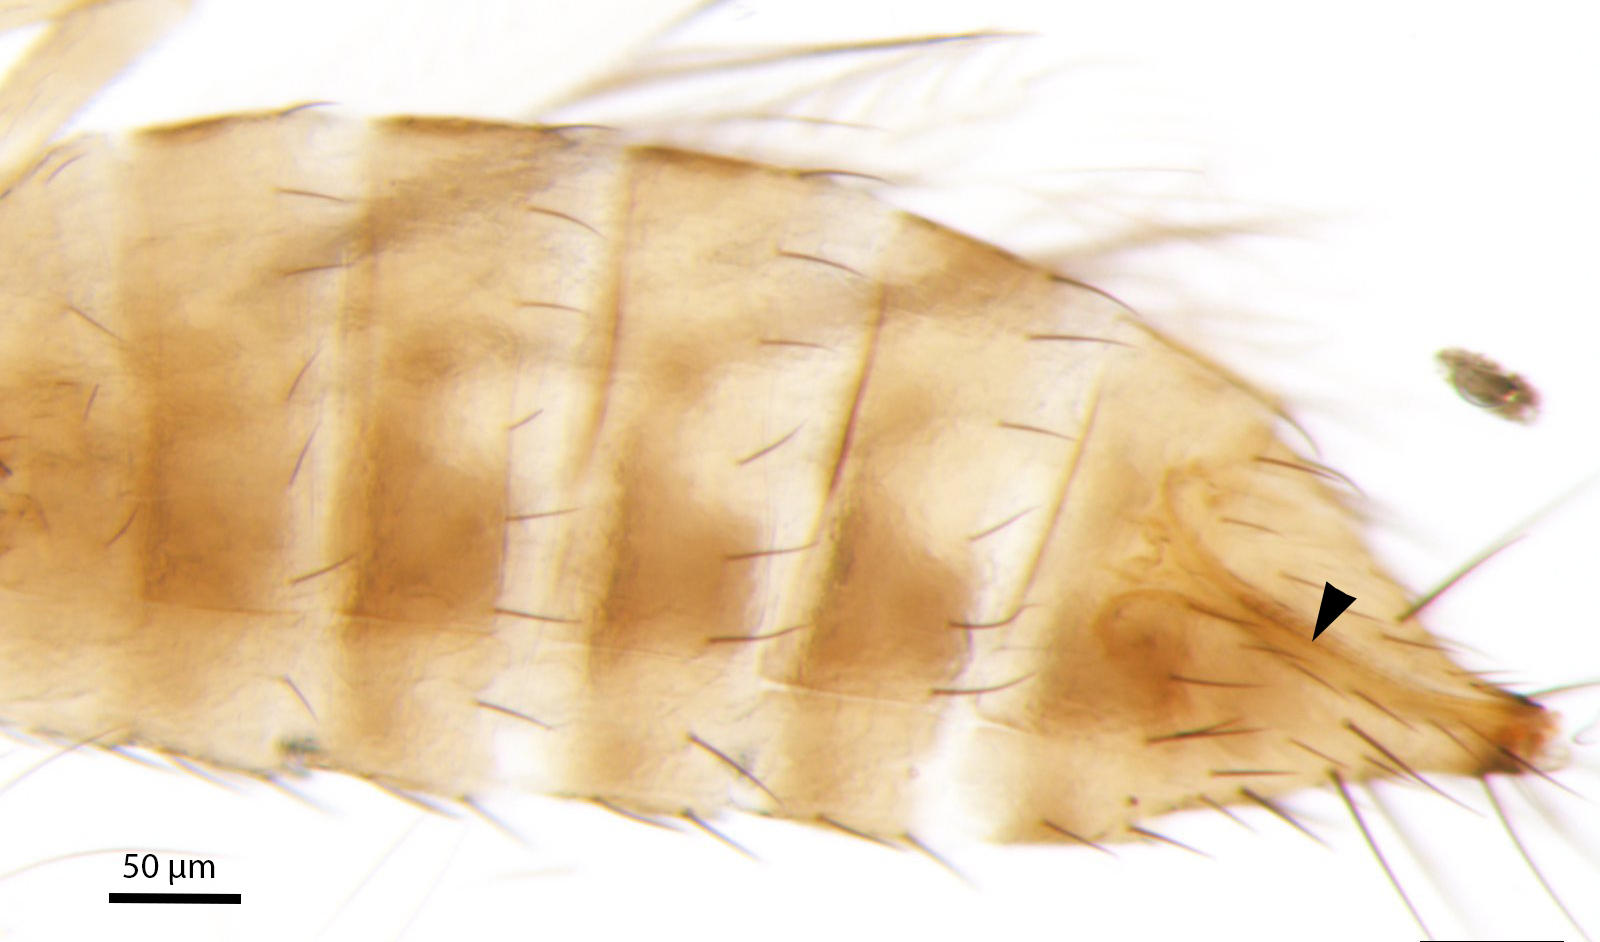
\includegraphics[width=\textwidth]{ThripidOvip}
  \caption{Ventral view of abdomen and ovipositor (arrow). Photo (CC BY 2.0) by Istv\'an Mik\'o \url{https://flic.kr/p/yNznf5}}
  \label{fig:thripid2}
 \end{subfigure}
 \caption{Thripidae}\label{fig:thripid}
\end{figure}

\subsection{Tubulifera}
\subsubsection{Phlaeothripidae (tube-tailed thrips)}
\noindent{}\textit{Diagnostic characters:} terminal abdominal segment tubular, not divided ; ventrally, with parallel lateral margins (Figure \ref{fig:phlaeothripid2}); ovipositor absent; wings with short, bare longitudinal veins and no acanthae (Figure \ref{fig:phlaeothripid2}).\\

\noindent{}\textit{Natural history:} \\

\begin{figure}[ht!]
 \centering
 \begin{subfigure}[ht!]{0.5\textwidth}
  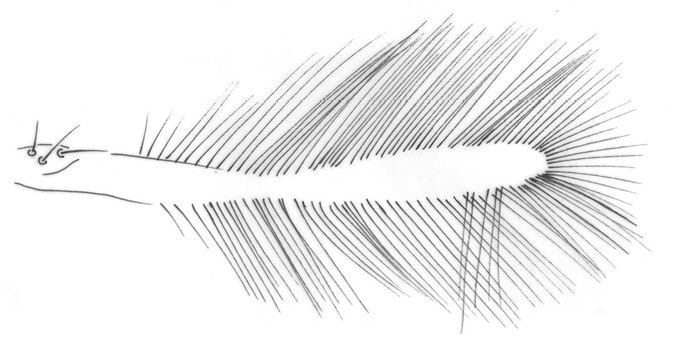
\includegraphics[width=\textwidth]{PhlaeothripidWing}
  \caption{Fore wing \citep[][Fig. 6]{minaei2013}}
  \label{fig:phlaeothripid1}
 \end{subfigure}
 \qquad
 \begin{subfigure}[ht!]{0.3\textwidth}
  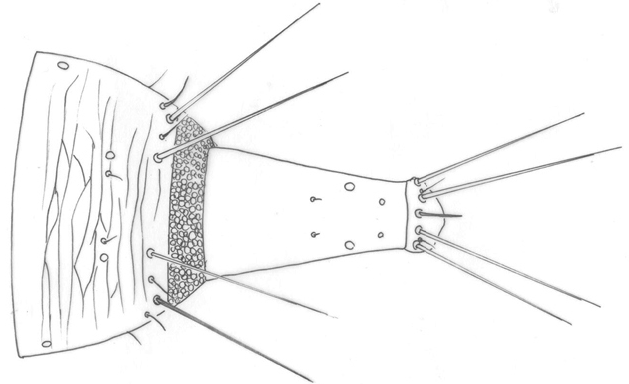
\includegraphics[width=\textwidth]{PhlaeothripidAbdomen}
  \caption{Dorsal view of abdomen apex \citep[][Fig. 9]{minaei2013}}
  \label{fig:phlaeothripid2}
 \end{subfigure}
 \caption{Phlaeothripidae}\label{fig:phlaeothripids}
\end{figure}

\section{Hemiptera (true bugs, scale insects, aphids, hoppers, etc.)}
\noindent{}\textit{Diagnostic characters:} antenna usually with 5--10 antennomeres, sometimes reduced; piercing/sucking mouthpart (mandible and maxillae rod-like stylets); labium elongate, multi-segmented and surrounds the stylets posteriorly (beak); prothorax is usually wider than long; fore wing is sometimes more sclerotized than hind wing (\textit{e.g.}, Heteroptera); arolium (apicomedial membraneous area of pretarsus) balloon shaped, often exceeds tarsal claw apically, sometimes absent, not eversible; cercus absent.\\

\subsection{Sternorrhyncha (psyllids, whiteflies, aphids, scale insects)}
\noindent{}\textit{Diagnostic characters:} tarsi 1- or 2-segmented; antennae filiform, sometimes absent labium arises from the head in between the procoxae when the head is in normal position, sometimes reduced; ovipositor reduced.\\

\subsubsection{Psyllidae (jumping plantlice)}
\noindent{}\textit{Diagnostic characters:} tarsi 2-segmented; antennae 5--10-segmented (usually 10); fore wings often more sclerotized than hind wing.

\noindent{}\textit{Natural history:} \\

\begin{figure}[ht!]
 \centering
 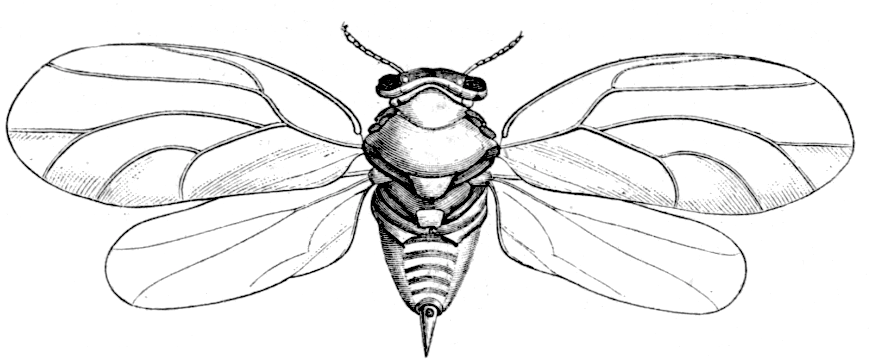
\includegraphics[width=0.55\textwidth]{PsyllidHabitus}
 \caption{Psyllidae habitus \citep[][Fig. 10d]{bhlpart17516}}
 \label{fig:psyllid}
\end{figure}

\subsubsection{Aphididae (aphids)}
\noindent{}\textit{Diagnostic characters:} tarsi 2-segmented, antennae usually 6-segmented; hind wing much smaller than fore wings; cornicles present near posterior end of abdomen (Figure \ref{fig:aphid1}).\\

\noindent{}\textit{Natural history:} \\

\begin{figure}[ht!]
 \centering
 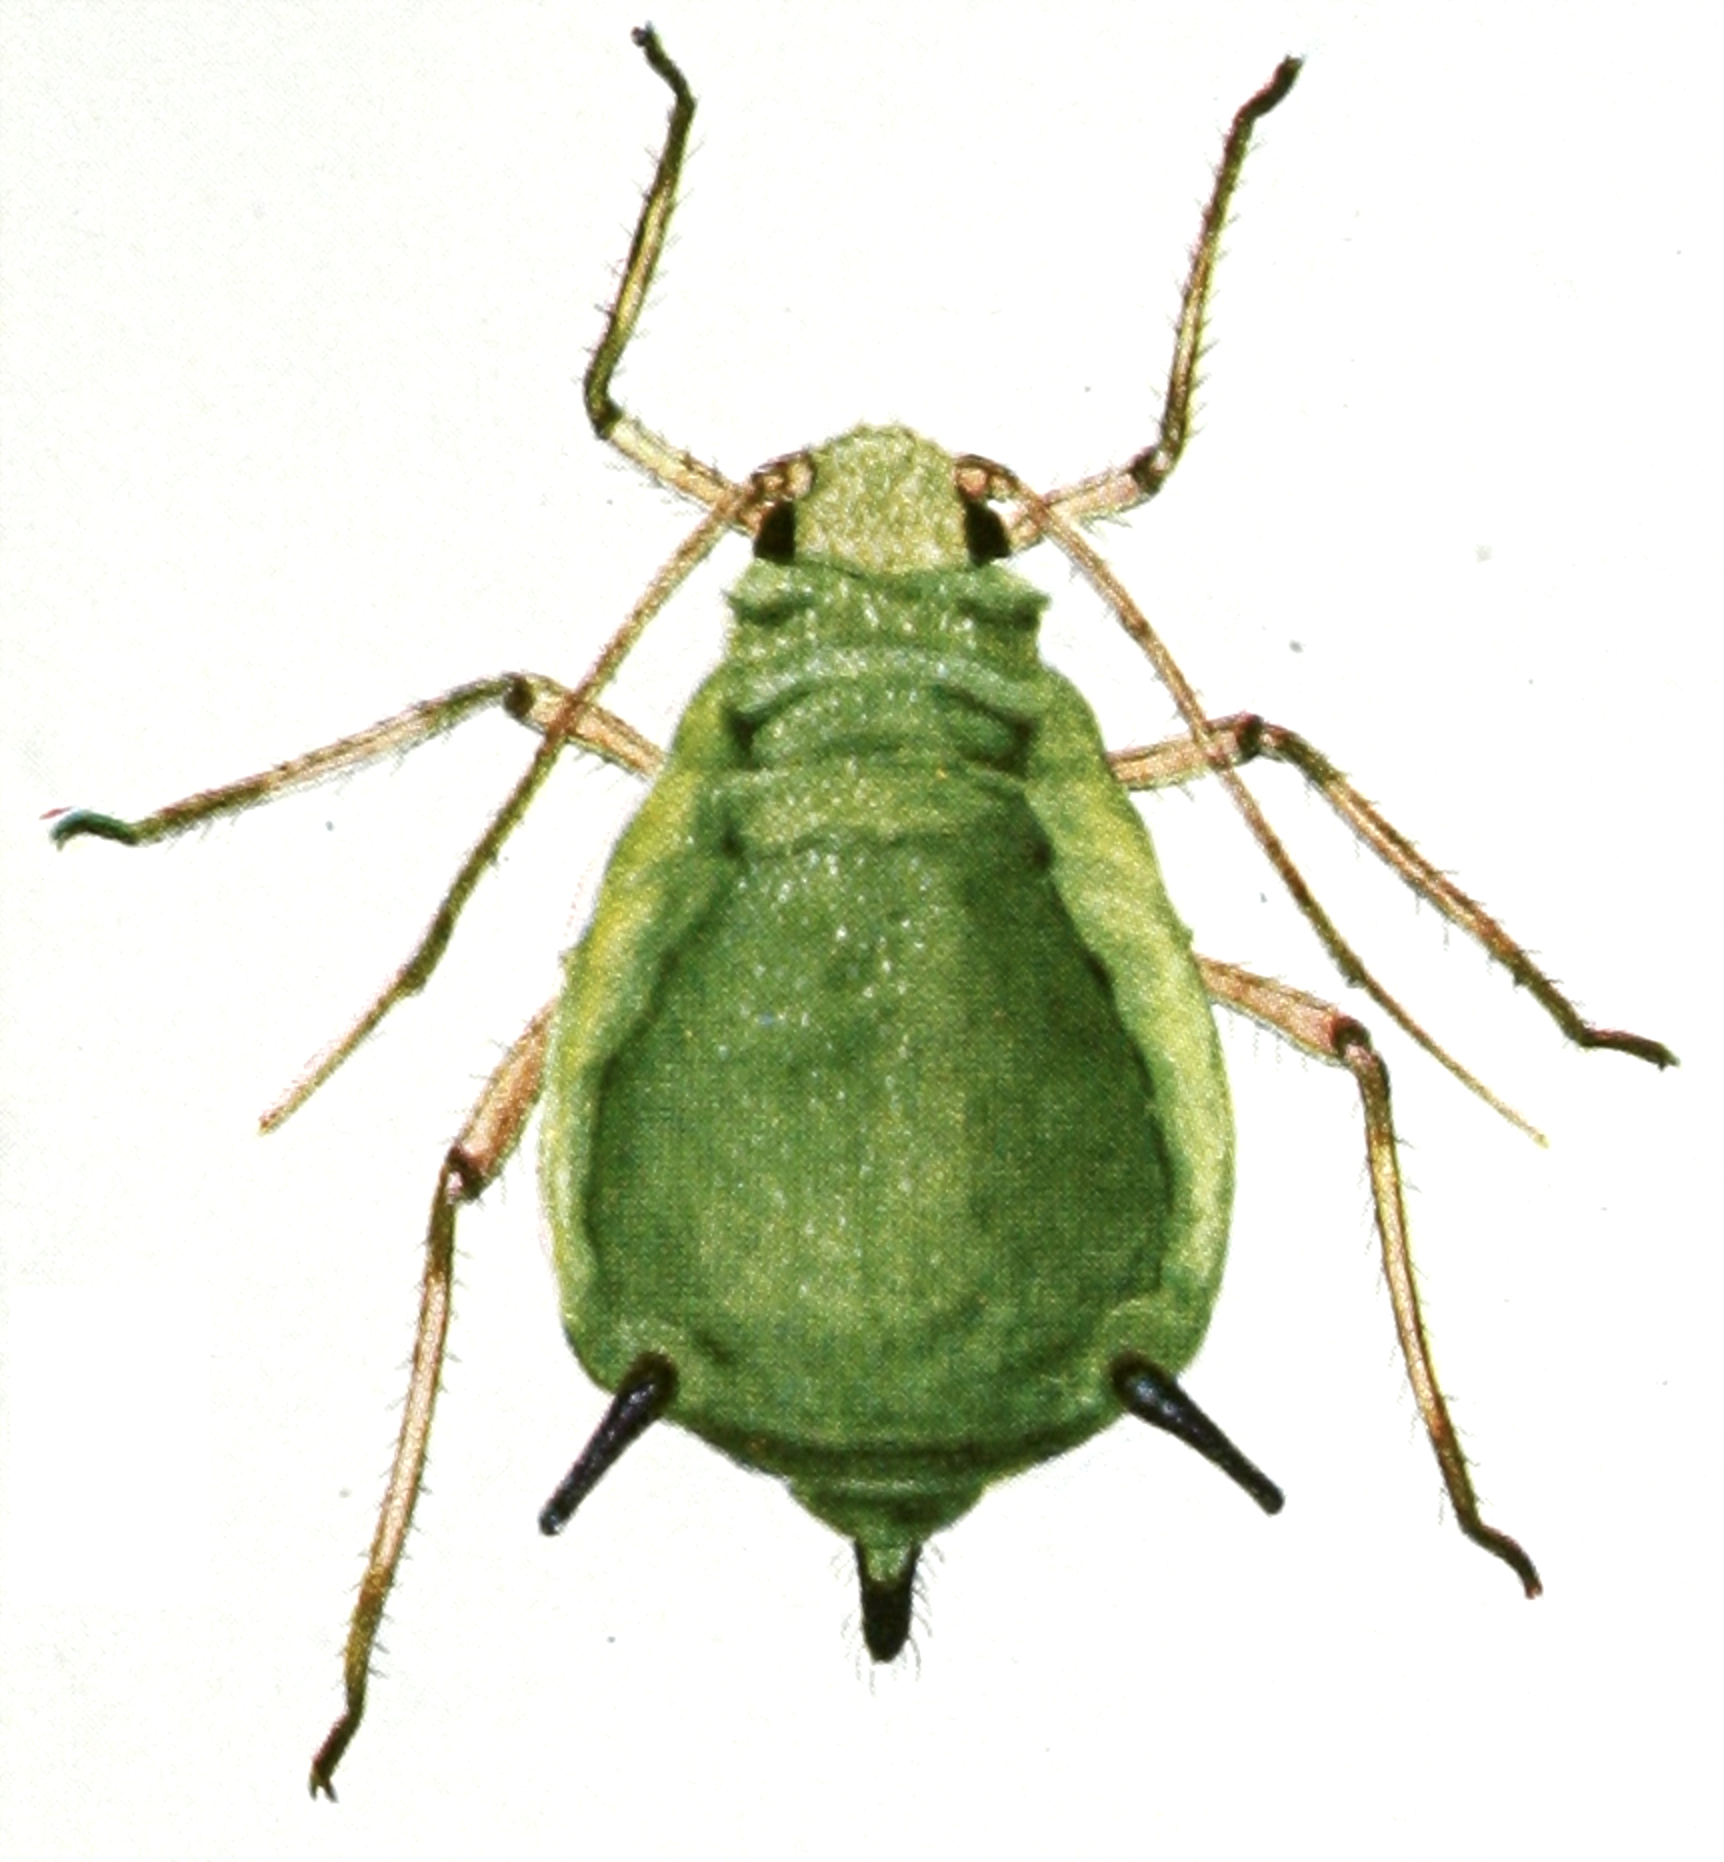
\includegraphics[width=0.35\textwidth]{AphididHabitus}
 \caption{Aphididae habitus (\citep[][Plate IIA]{bhl128276}}
 \label{fig:aphid1}
\end{figure}

\subsubsection{Aleyrodidae (whiteflies)}
\noindent{}\textit{Diagnostic characters:} tarsi 2-segmented, antennae 7-segmented (Figure \ref{fig:aleyrodid1}); hind wing almost as large as fore wings; wings held horizontally over body while at rest; body and wings covered with white powder (depends on preservation) (Figure \ref{fig:aleyrodid2}).\\

\noindent{}\textit{Natural history:} \\

\noindent{}What is the function of the white ``powder'' that covers their bodies? How would you test your hypothesis? \vspace{4cm}

\begin{figure}[ht!]
 \centering
 \begin{subfigure}[ht!]{0.45\textwidth}
  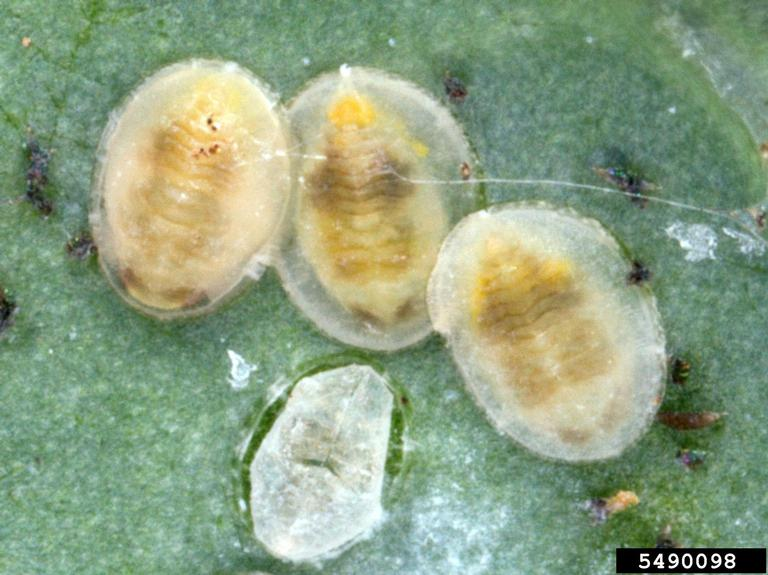
\includegraphics[width=\textwidth]{AleyrodidNymph}
  \caption{Dorsal habitus, nymph. Photo (CC BY-NC 3.0) by David Cappaert \url{http://goo.gl/FvsQqt}}
  \label{fig:aleyrodid1}
 \end{subfigure}
 \qquad
 \begin{subfigure}[ht!]{0.45\textwidth}
  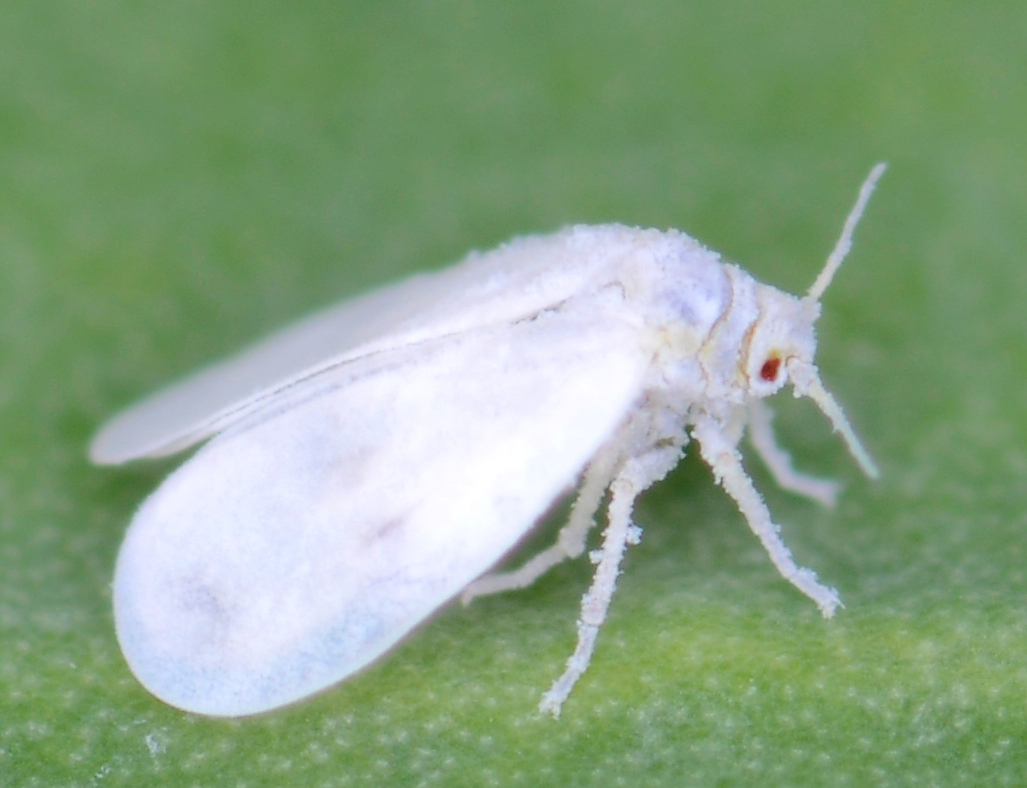
\includegraphics[width=\textwidth]{AleyrodidHabitus}
  \caption{Lateral habitus. Photo (CC BY-SA 4.0) by Amada44 \url{https://goo.gl/chHgyt}}
  \label{fig:aleyrodid2}
 \end{subfigure}
 \caption{Aleyrodidae}\label{fig:aleyrodid}
\end{figure}

\noindent{}The following families are classified in \textbf{Coccoidea}, commonly referred to as scale insects. They share the following characteristics: adult males winged, 1-segmented tarsi (rarely 2), 1 pair of wings, no beak; females always wingless, sometimes legless or nearly so, often with a waxy or scale-like covering; first instar nymphs (``crawlers'') are quite mobile and have distinct legs and antennae.\\

\noindent{}These insects also live primarily sedentary lives, with virtually no locomotion after the first instar, ``crawler'' stage (at least for females). As you examine these scale specimens, think about their adaptations to this kind of lifestyle. \\

\subsubsection{Pseudococcidae (mealybugs)}
\noindent{}\textit{Diagnostic characters:} body ovular, usually with a powdery waxy coating; terminal abdominal segments, anal opening with setae; have well developed legs.\\%???

\noindent{}\textit{Natural history:} \\

\begin{figure}[ht!]
 \centering
 \begin{subfigure}[ht!]{0.38\textwidth}
  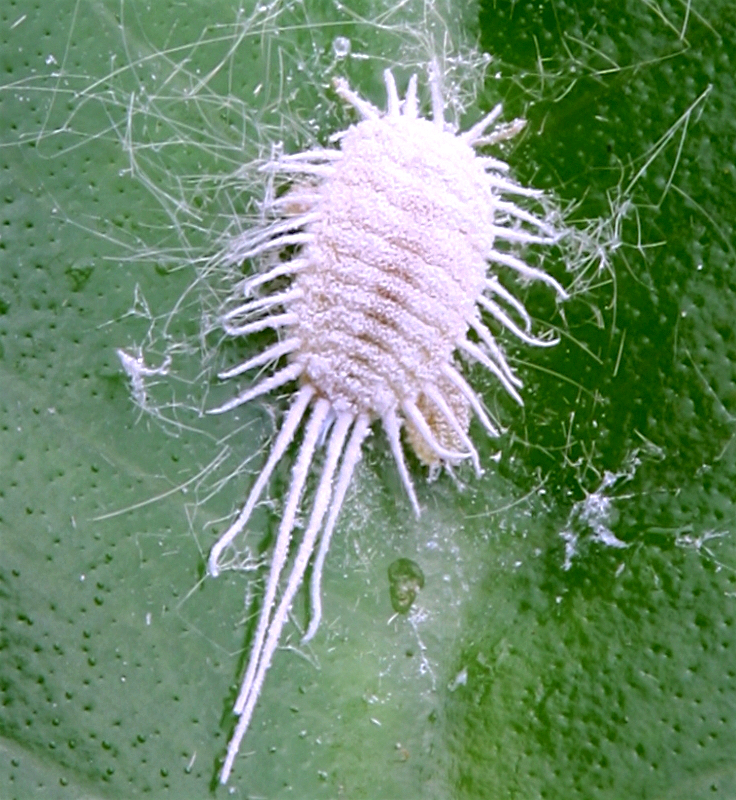
\includegraphics[width=\textwidth]{PseudococcidDorsalHabitus}
  \caption{Dorsal habitus. Photo (CC BY-SA 3.0 AT) by D-Kuru \url{https://goo.gl/1tsXbc}}
  \label{fig:pseudococcid1}
 \end{subfigure}
 \qquad
 \begin{subfigure}[ht!]{0.45\textwidth}
  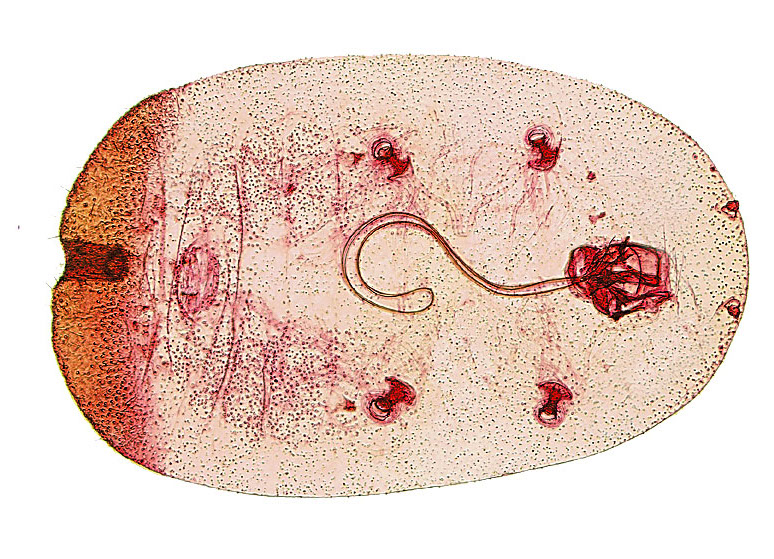
\includegraphics[width=\textwidth]{PseudococcidHabitus}
  \caption{Ventral habitus (image from \cite{ScaleNet})}
  \label{fig:pseudococcid2}
 \end{subfigure}
 \caption{Pseudococcidae}\label{fig:pseudococcid}
\end{figure}

\subsubsection{Monophlebidae (giant scale insects)}
\noindent{}\textit{Diagnostic characters:} adult female flattened or spherical, often cylindrical or scalloped, with hard covering formed of wax and cast skins of earlier instars abdominal spiracles present; female antennae short or long, up to 13 segments, no wings or legs.\\

\noindent{}\textit{Natural history:} \\

\begin{figure}[ht!]
 \centering
 \begin{subfigure}[ht!]{0.42\textwidth}
  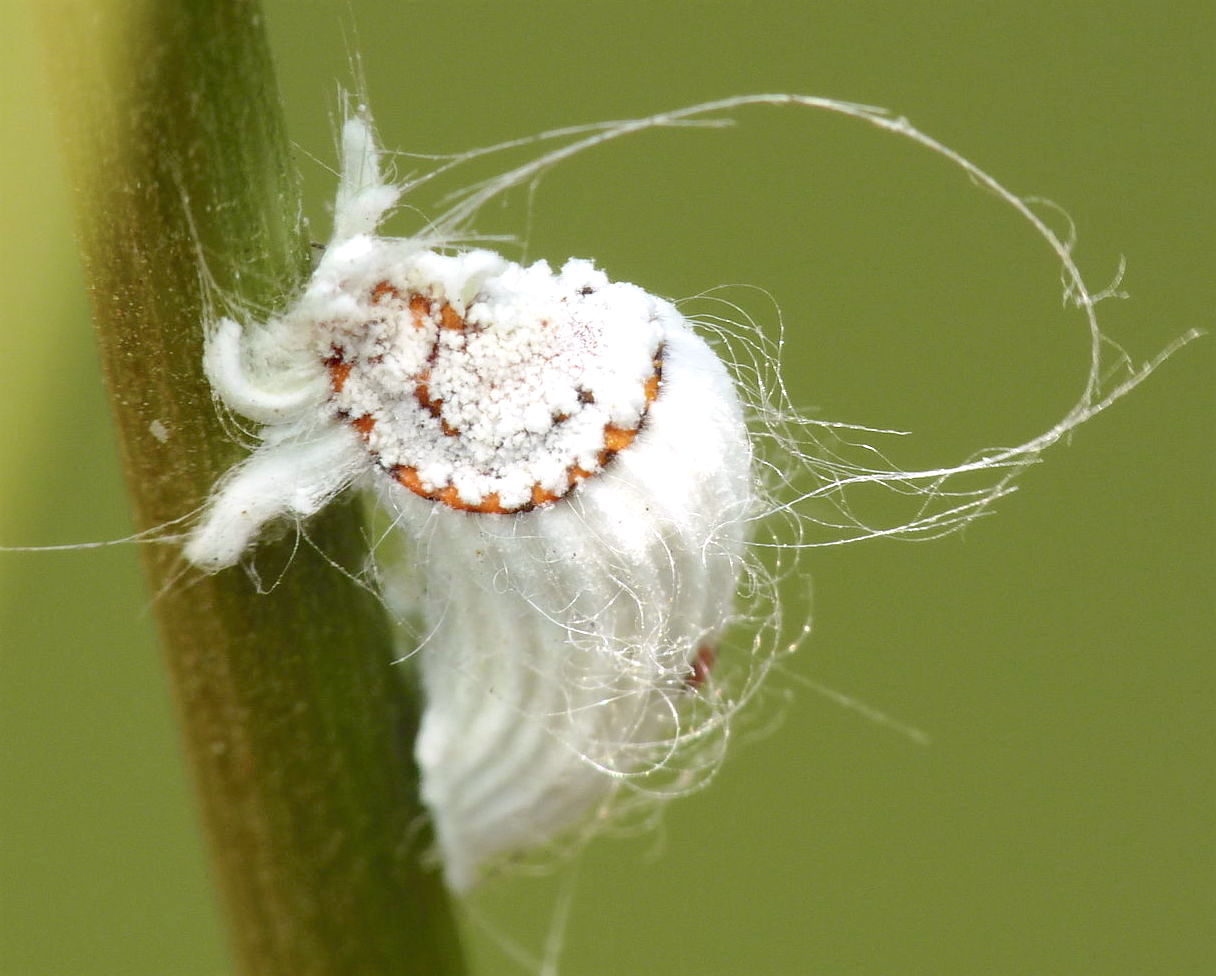
\includegraphics[width=\textwidth]{MonophlebidDorsalHabitus}
  \caption{Dorsal habitus. Photo (CC BY-SA 3.0) by Lucarelli \url{https://goo.gl/dQNTNy}}
  \label{fig:monophlebid1}
 \end{subfigure}
 \qquad
 \begin{subfigure}[ht!]{0.45\textwidth}
  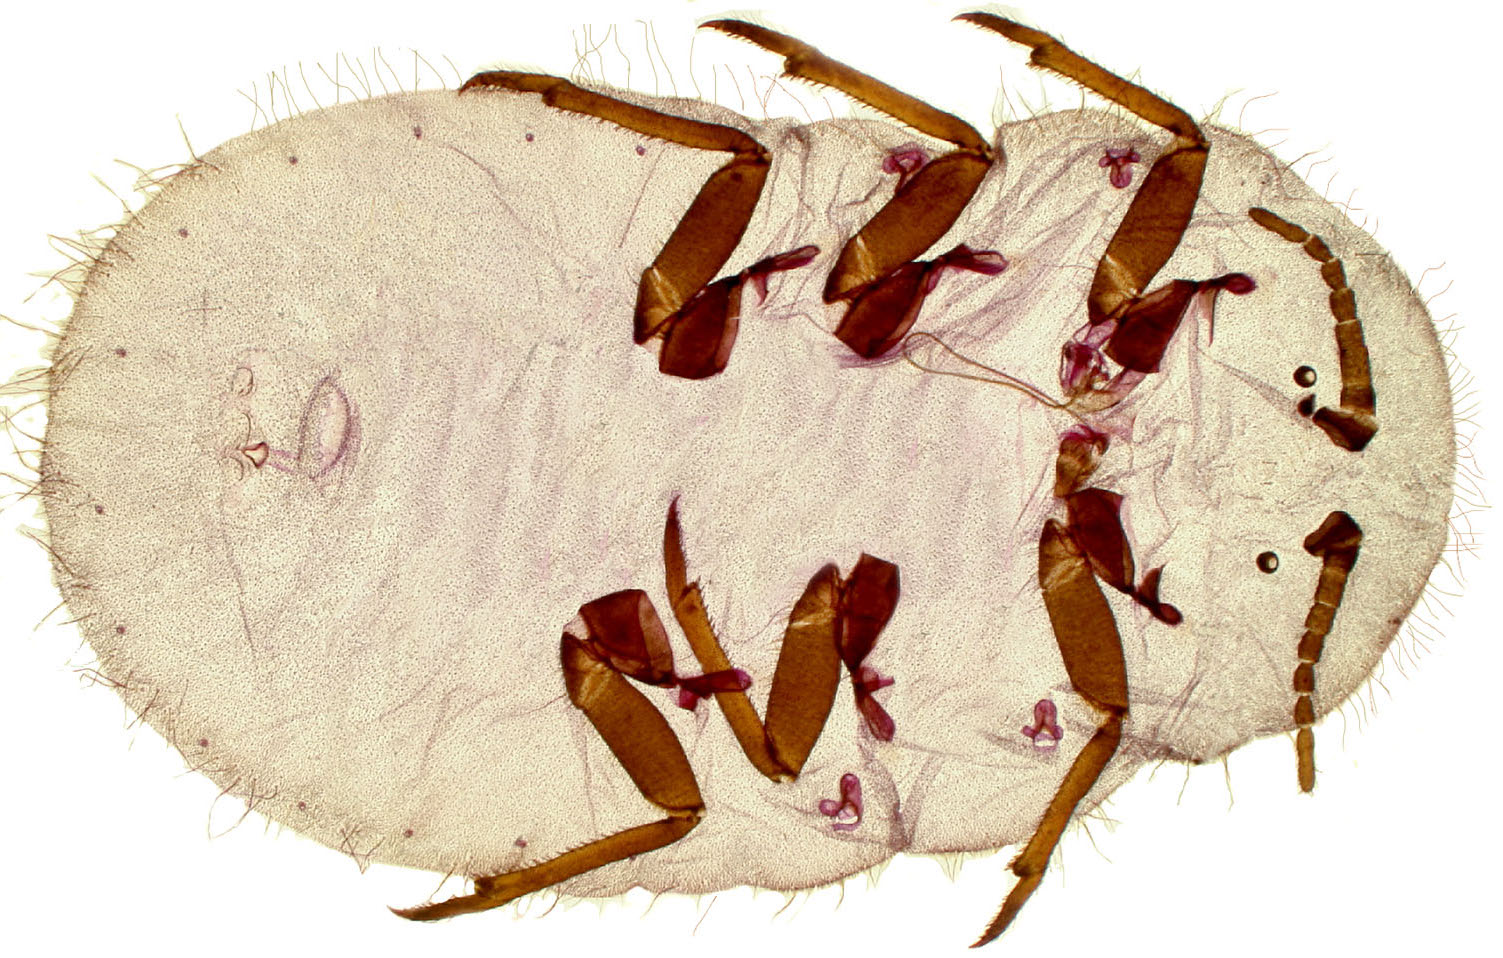
\includegraphics[width=\textwidth]{MonophlebidHabitus}
  \caption{Ventral habitus (image from \cite{ScaleNet})}
  \label{fig:monophlebid2}
 \end{subfigure}
 \caption{Monophlebidae}\label{fig:monophlebids}
\end{figure}

\subsubsection{Coccidae (soft scale insects, wax and tortoise scales)}
\noindent{}\textit{Diagnostic characters:} adult female flattened and oval with smooth, hard exoskeleton or soft waxy covering (Figure \ref{fig:coccid2}); 2 triangular plates on anal opening; abdomen with anal cleft; legs often present but reduced; antennae reduced or absent.\\

\noindent{}\textit{Natural history:} \\

\begin{figure}[ht!]
 \centering
 \begin{subfigure}[ht!]{0.45\textwidth}
  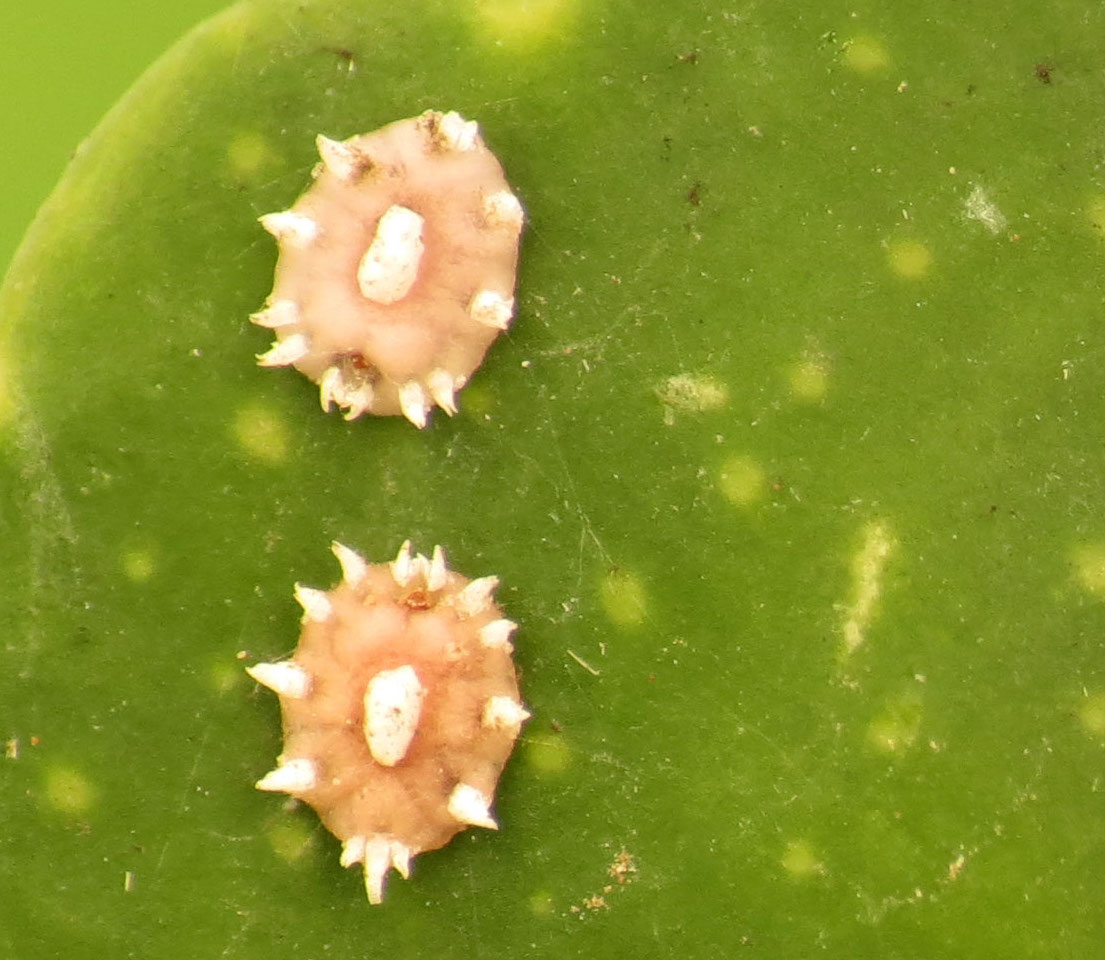
\includegraphics[width=\textwidth]{CoccidDorsalHabitus}
  \caption{Dorsal habitus. Photo (CC BY 2.0) by Katja Schulz \url{https://flic.kr/p/qLWfyn}}
  \label{fig:coccid1}
 \end{subfigure}
 \qquad
 \begin{subfigure}[ht!]{0.45\textwidth}
  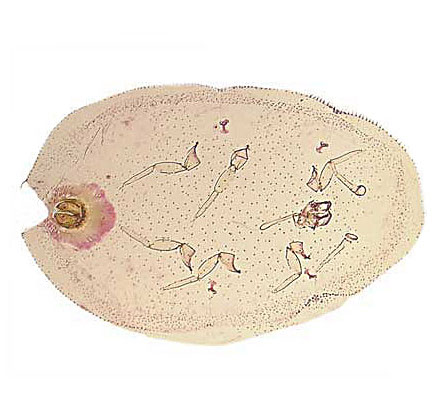
\includegraphics[width=\textwidth]{CoccidHabitus}
  \caption{Ventral habitus (image from \cite{ScaleNet})}
  \label{fig:coccid2}
 \end{subfigure}
 \caption{Coccidae}\label{fig:coccid}
\end{figure}

\subsubsection{Diaspididae (armored scale insects)}
\noindent{}\textit{Diagnostic characters:} adult female flattened, disc-like with hard covering formed of wax and cast skins of earlier instars; terminal abdominal segments form fused pygidium, anal opening without setae; antennae, wings, and legs lacking.\\

\noindent{}\textit{Natural history:} \\

\begin{figure}[ht!]
 \centering
 \begin{subfigure}[ht!]{0.45\textwidth}
  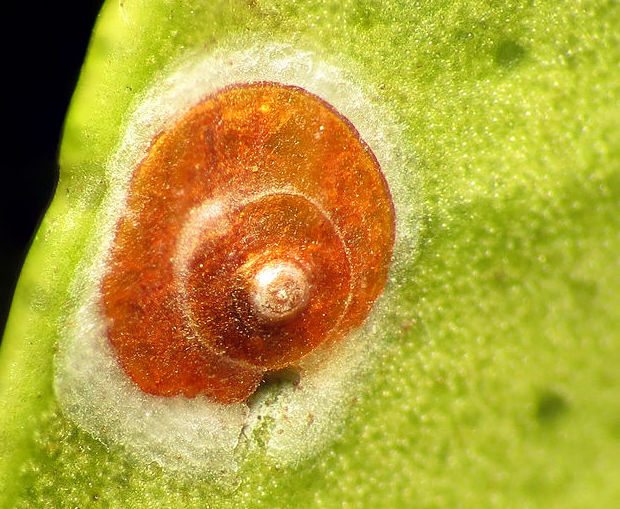
\includegraphics[width=\textwidth]{DiaspididDorsalHabitus}
  \caption{Dorsal habitus. Photo (CC BY 2.0) by Katja Schulz \url{https://flic.kr/p/CB5WCU}}
  \label{fig:diaspidid1}
 \end{subfigure}
 \qquad
 \begin{subfigure}[ht!]{0.45\textwidth}
  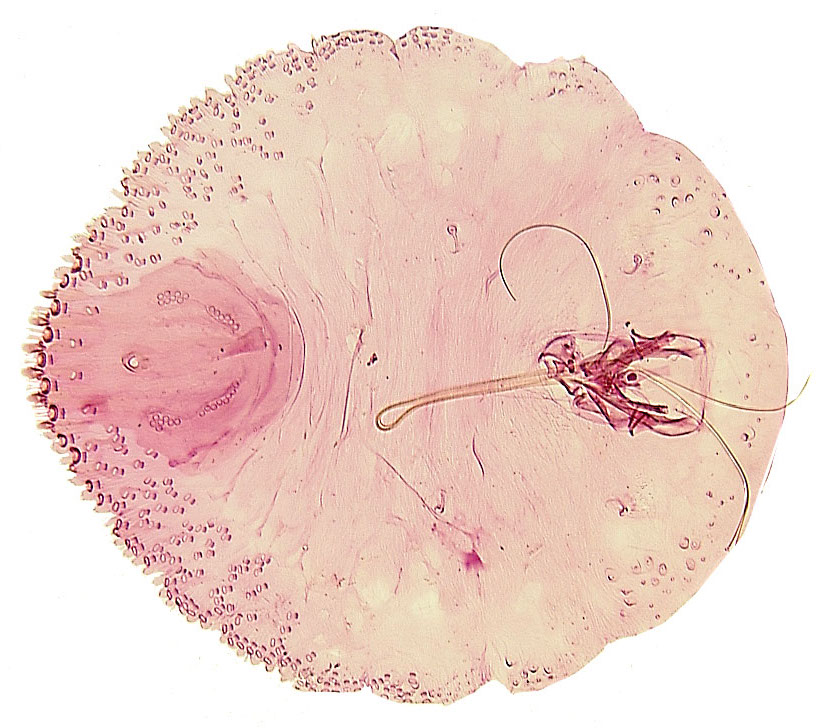
\includegraphics[width=\textwidth]{DiaspididHabitus}
  \caption{Ventral habitus (image from \cite{ScaleNet})}
  \label{fig:diaspidid2}
 \end{subfigure}
 \caption{Diaspididae}\label{fig:diaspidid}
\end{figure}

\noindent{}Describe three adaptions you observed in these insects that allow them to live in one location for most of their lives. What challenges does this life history present?\\

\subsection{Auchenorrhyncha (cicadas, hoppers)}
\noindent{}\textit{Diagnostic characters:} head hypognathous, mouthparts arises posteroventrally from head; labium arises from the head anterior to the procoxae when the head is in normal position; antennae aristate; fore wing is not more sclerotized as hind wing; tarsi 3-segmented; presence of a complex tymbal acoustic system on abdominal segment I; ovipositor well developed.\\

\subsubsection{Cicadidae (cicadas)}
\noindent{}\textit{Diagnostic characters:} relatively large (\textgreater{}2 cm); antennae arise between compound eyes that are widely separated (Figure \ref{fig:cicadidae}); hind tibiae without large apical spur (\textit{i.e.}, a moveable projection); hind tibia without robust lateral and apical spines; tymbals present.\\

\noindent{}\textit{Natural history:} \\

\noindent{}Tymbals are present in all Auchenorrhyncha, but they are easy to see in Cicadidae due to their large size. Can you find and sketch them?

\begin{figure}[ht!]
 \centering
 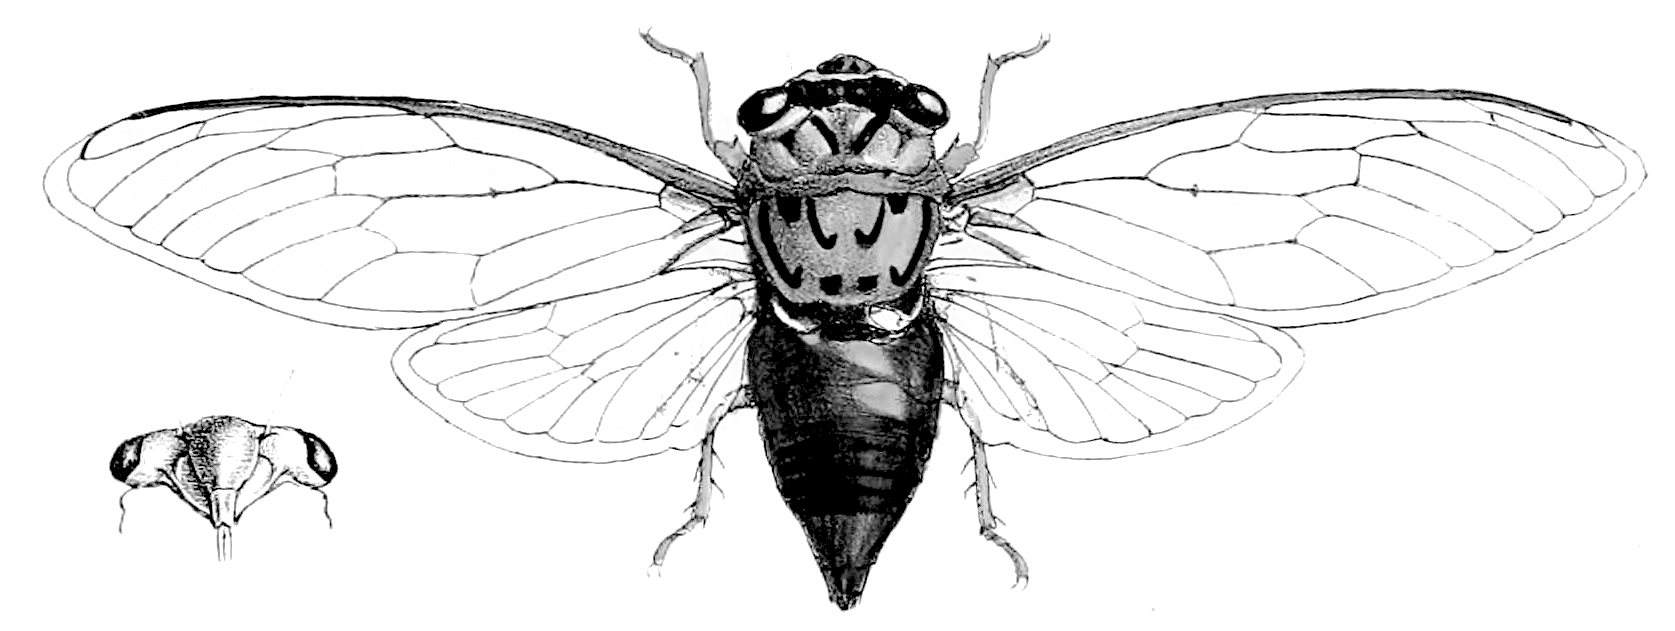
\includegraphics[width=0.75\textwidth]{CicadidHabitus}
 \caption{Cicadidae habitus \citep[][Plate 100]{bhl33187}}
 \label{fig:cicadidae}
\end{figure}

\subsubsection{Membracidae (treehoppers)}
\noindent{}\textit{Diagnostic characters:} pronotum extends over abdomen; fore wing without many costal crossveins (Figure \ref{fig:membrac2}; compare to Cicadidae); hind tibiae without large apical spur and without faint lateral spines.\\

\noindent{}\textit{Natural history:} \\

\begin{figure}[ht!]
 \centering
 \begin{subfigure}[ht!]{0.45\textwidth}
  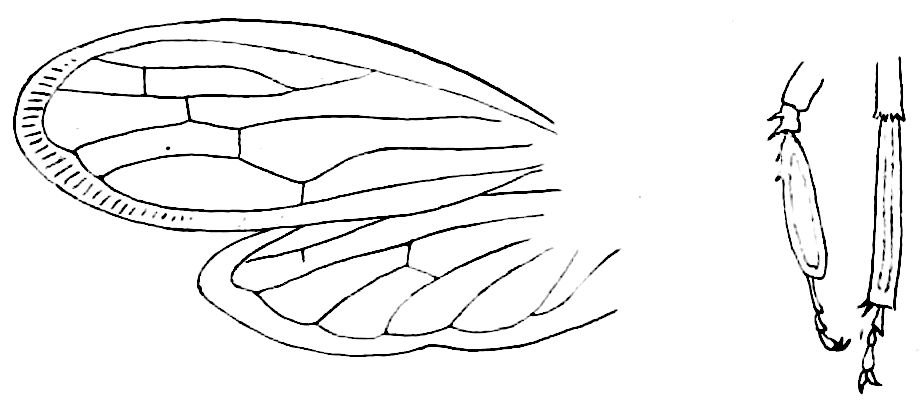
\includegraphics[width=\textwidth]{MembracidWings}
  \caption{Wings and legs \citep[][Plate I, Figs. 4c,4e]{bhl79792}}
  \label{fig:membrac1}
 \end{subfigure}
 \qquad
 \begin{subfigure}[ht!]{0.45\textwidth}
  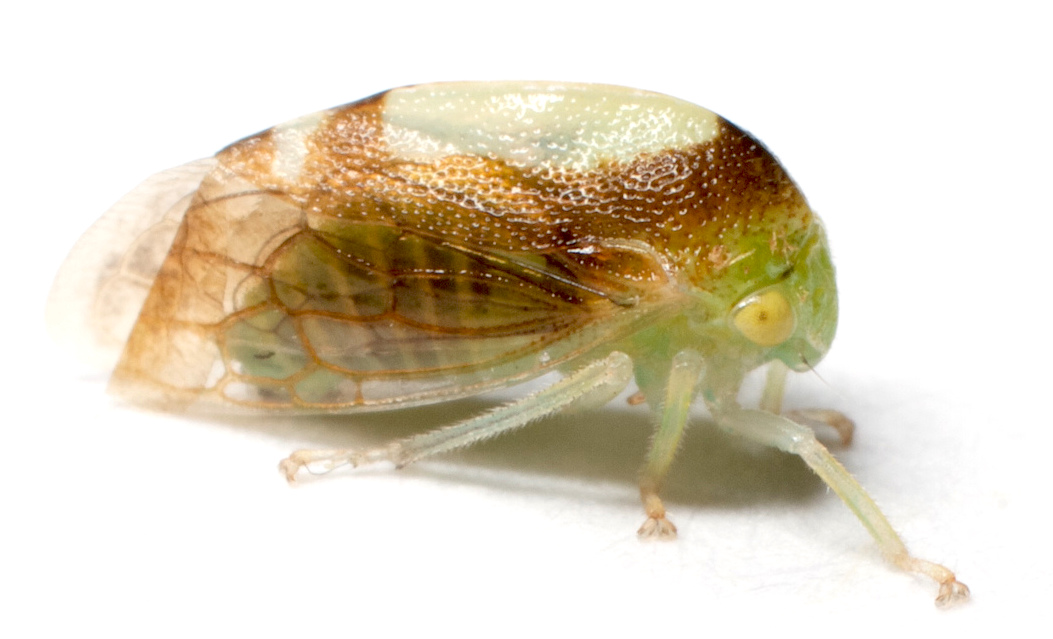
\includegraphics[width=\textwidth]{MembracidHabitus}
  \caption{Habitus. Photo (CC By 2.0) by Brian Gratwicke \url{https://flic.kr/p/rGLMDm}}
  \label{fig:membrac2}
 \end{subfigure}
 \caption{Membracidae}\label{fig:membracid}
\end{figure}

\subsubsection{Cicadellidae (leafhoppers)}
\noindent{}\textit{Diagnostic characters:} pronotum does not extend over abdomen (Figure \ref{fig:cicadellids}); hind tibia with two rows of slender, elongate spines.\\

\noindent{}\textit{Natural history:} \\

\begin{figure}[ht!]
 \centering
 \begin{subfigure}[ht!]{0.4\textwidth}
  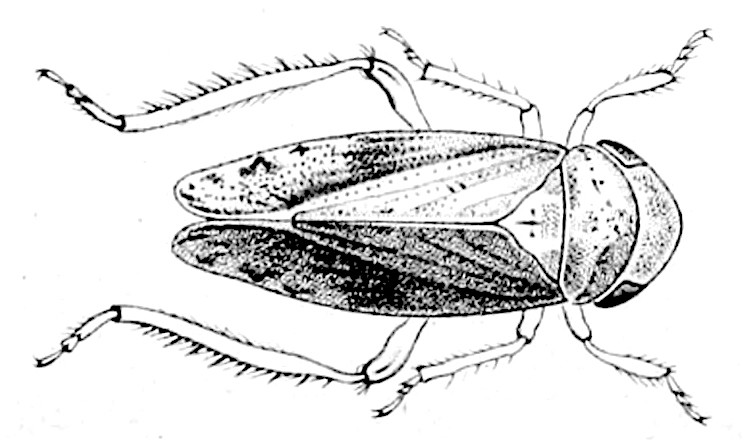
\includegraphics[width=\textwidth]{CicadellidHabitusInk}
  \caption{Habitus \citep[][Plate 8, Fig. 16]{bhl37902}}
  \label{fig:cicadellid1}
 \end{subfigure}
 \qquad
 \begin{subfigure}[ht!]{0.45\textwidth}
  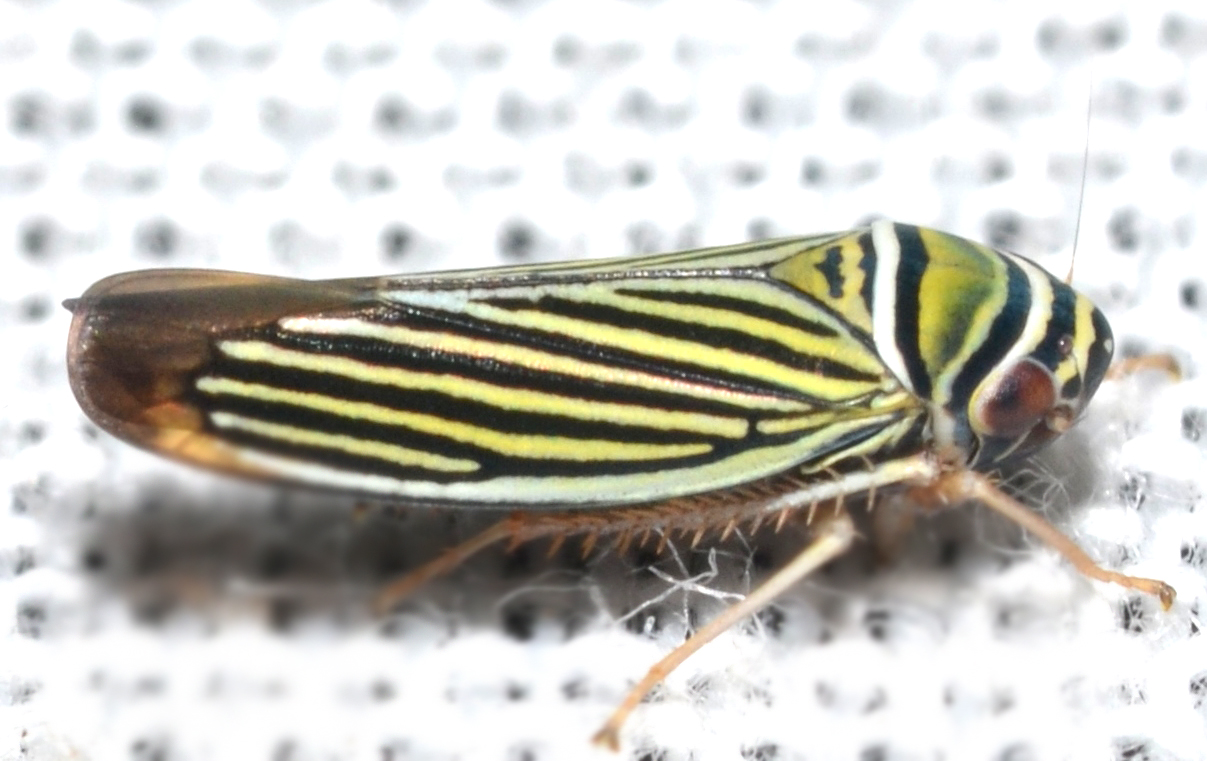
\includegraphics[width=\textwidth]{CicadellidHabitus}
  \caption{Habitus. Photo (CC BY 2.0) by Andy Reago \& Chrissy McClarren \url{https://flic.kr/p/xMeWGS}}
  \label{fig:cicadellid2}
 \end{subfigure}
 \caption{Cicadellidae}\label{fig:cicadellids}
\end{figure}

\subsubsection{Cercopidae (froghoppers, spittlebugs)}
\noindent{}\textit{Diagnostic characters:} hind tibiae with 1 or 2 robust lateral and numerous apical spines (Figure \ref{fig:cercopid}); fore wing usually more strongly sclerotized than hind wing.\\

\noindent{}\textit{Natural history:} \\

\begin{figure}[ht!]
 \centering
 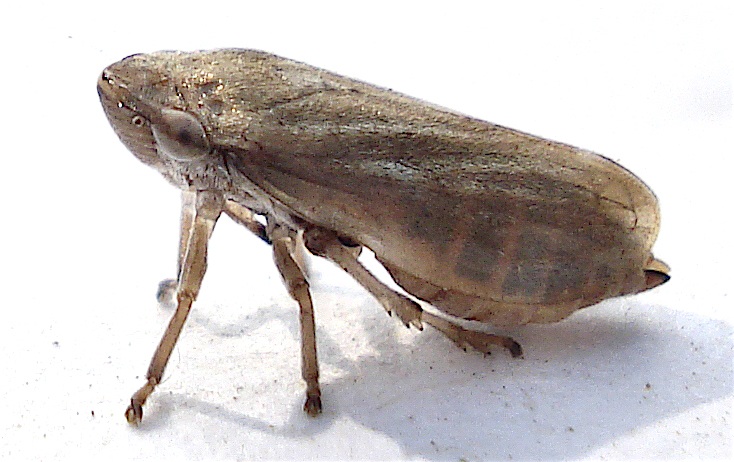
\includegraphics[width=0.45\textwidth]{CercopidHabitus}
 \caption{Cercopidae habitus. Photo (CC BY 2.0) by Mick Talbot \url{https://flic.kr/p/5nSL3i}}
 \label{fig:cercopid}
\end{figure}

\noindent{}\textit{Natural history:} \\

\subsubsection{Delphacidae}
\noindent{}\textit{Diagnostic characters:} Antennae arise below eyes on sides of head; median, emarginated area of the head present; fore wings without many costal crossveins; hind tibia with large apical spur (movable projection) (Figure \ref{fig:delphacids}).\\

\noindent{}\textit{Natural history:} \\

\begin{figure}[ht!]
 \centering
 \begin{subfigure}[ht!]{0.4\textwidth}
  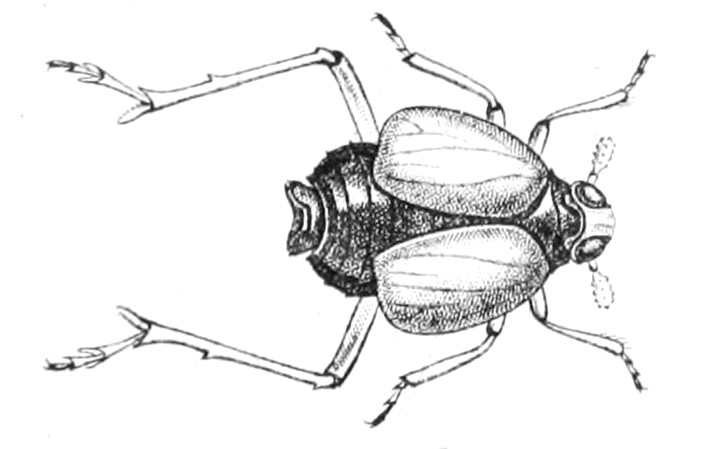
\includegraphics[width=\textwidth]{DelphacidHabitusInk}
  \caption{Habitus \citep[][Plate 7, Fig. 10]{bhl37902}}
  \label{fig:delphacid1}
 \end{subfigure}
 \qquad
 \begin{subfigure}[ht!]{0.45\textwidth}
  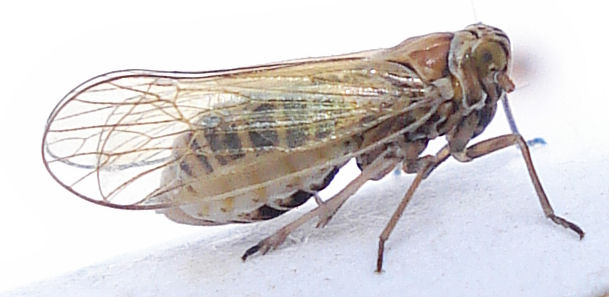
\includegraphics[width=\textwidth]{DelphacidHabitus}
  \caption{Habitus. Photo (CC BY 2.0) by Mick Talbot \url{https://flic.kr/p/6FYvWv}}
  \label{fig:delphacid2}
 \end{subfigure}
 \caption{Delphacidae}\label{fig:delphacids}
\end{figure}

\subsection{Heteroptera}
A suborder of Hemiptera commonly referred to as ``true bugs'', which can be recognized by the following characters:

\noindent{}\textit{Diagnostic characters:} head prognathous, mouthparts arises anteriorly from head
in lateral view, there is a distinct distance between the labium and the procoxae, compared to other hemipterans; antennae filiform; anterior part of fore wing is more sclerotized than posterior part of fore wing and the hind wing (hemelytra); tarsi with usually 3 tarsomeres, rarely 2 or 4 ; absence of a complex tymbal acoustic system on abdominal segment I; scent gland (sgo) on the metathorax usually present (but see Rhopalidae).\\

\noindent{}See Figure \ref{fig:anatomy} for general anatomical terms used by heteropterists.\\

\begin{figure}[ht!]
 \centering
 
\includegraphics[width=0.7\textwidth]{image14}
 \caption{cl=clavius, cor=corium, cun=cuneus, scl=scutellum, n1=pronotum (dorsal region of prothorax), ver=vertex, mem=membrane, ts=tarsus, tcl=tarsal claw, aro=arolium, sgo=scent gland opening, pl1=propleuron (lateral region of the prothorax), spr=spiracle}
 \label{fig:anatomy}
\end{figure}

\subsubsection{Enicocephalidae (unique-headed bugs)}
\noindent{}Specimens of this family, which is thought to be sister to the rest of Heteroptera, can be found in glycerol: \url{http://www.gigapan.com/gigapans/164037}. What makes the head of this bug unique?\vspace{3cm}

\begin{figure}[ht!]
 \centering
 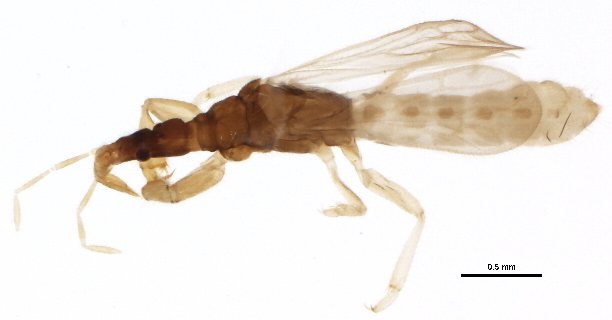
\includegraphics[width=0.5\textwidth]{EnicocephalidHabitus}
 \caption{Enicocephalidae habitus. Photo (CC BY-NC-SA 3.0) by BIO Photography Group, Biodiversity Institute of Ontario \url{http://goo.gl/obSS2z}}
 \label{fig:enicocephalid}
\end{figure}

\subsubsection{Gelastocoridae (toad bugs)}
\noindent{}\textit{Diagnostic characters:} Body usually \textless{}10 mm long, toad-like, cryptic (camouflaged); antennae shorter than head, hidden; ocelli present; flattened, bulging eyes (Figure \ref{fig:gelasto1}); fore legs shorter than middle legs.\\

\noindent{}\textit{Natural history:} \\

\begin{figure}[ht!]
 \centering
 \begin{subfigure}[ht!]{0.35\textwidth}
  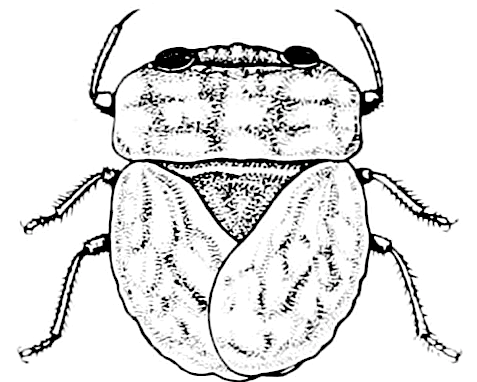
\includegraphics[width=\textwidth]{GelastocoridHabitusInk}
  \caption{Habitus \citep[][Plate XXXII, Fig. 10]{bhl82061}}
  \label{fig:gelasto1}
 \end{subfigure}
 \qquad
 \begin{subfigure}[ht!]{0.32\textwidth}
  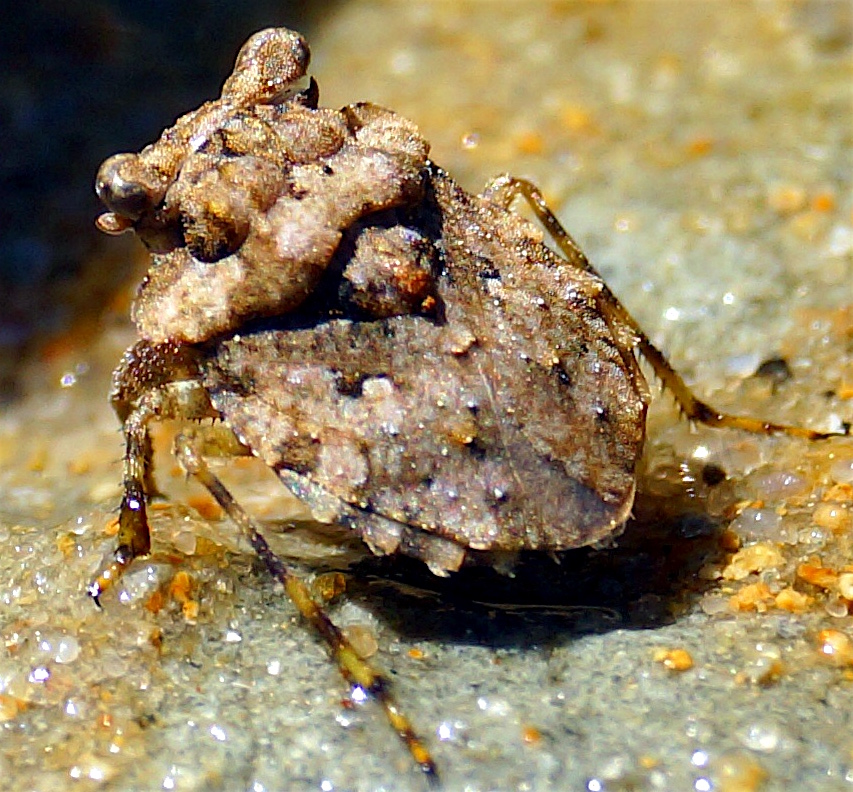
\includegraphics[width=\textwidth]{GelastocoridHabitus}
  \caption{Habitus. Photo (CC BY-SA 2.0) by dr.scott.mills \url{https://flic.kr/p/efgMcq}}
  \label{fig:gelasto2}
 \end{subfigure}
 \caption{Gelastocoridae}\label{fig:gelastocorids}
\end{figure}

\subsubsection{Corixidae (water boatmen)}
\noindent{}\textit{Diagnostic characters:} Body flattened dorsally, with dark pattern of thin stripes; antennae shorter than head; ocelli absent; beak very short, appears 1-segmented (Figure \ref{fig:corix1}); fore legs not raptorial, fore tarsi 1-segmented and scoop-shaped (Figure \ref{fig:corix1}); hind legs elongate, oar-like, hind tarsi without claws.\\

\noindent{}\textit{Natural history:} \\

\begin{figure}[ht!]
 \centering
 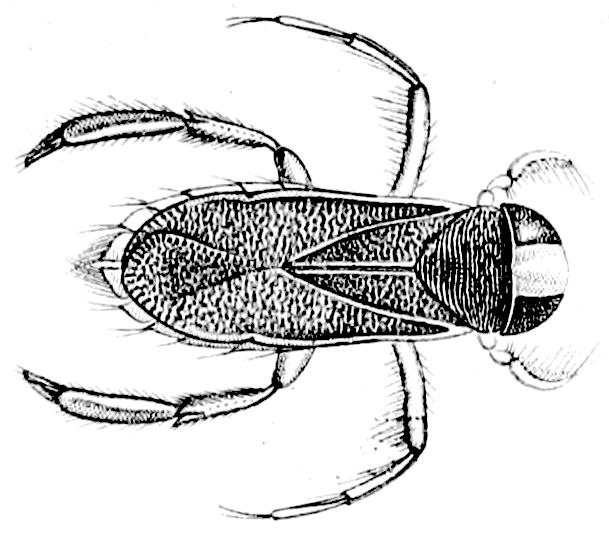
\includegraphics[width=0.35\textwidth]{CorixidHabitus}
 \caption{Corixidae dorsal habitus \citep[][Plate 7, Fig. 5]{bhl37902}}
 \label{fig:corix1}
\end{figure}

\noindent{}Compare the mouthparts of Corixidae to the other heteropterans. What do you think Corixidae eat, based on the morphology of the mouthparts? Hints: These are aquatic insects. Also, check out their fore legs.\vspace{2cm}

\subsubsection{Notonectidae (backswimmers)}
\noindent{}\textit{Diagnostic characters:} Body convex dorsally, mottled, light-colored (Figure \ref{fig:notonect1}); antennae shorter than head; ocelli absent; fore legs not raptorial, front tarsi not scoop-shaped; hind legs elongate, oar-like, hind tarsi without claws.\\

\noindent{}\textit{Natural history:} \\

\begin{figure}[ht!]
 \centering
 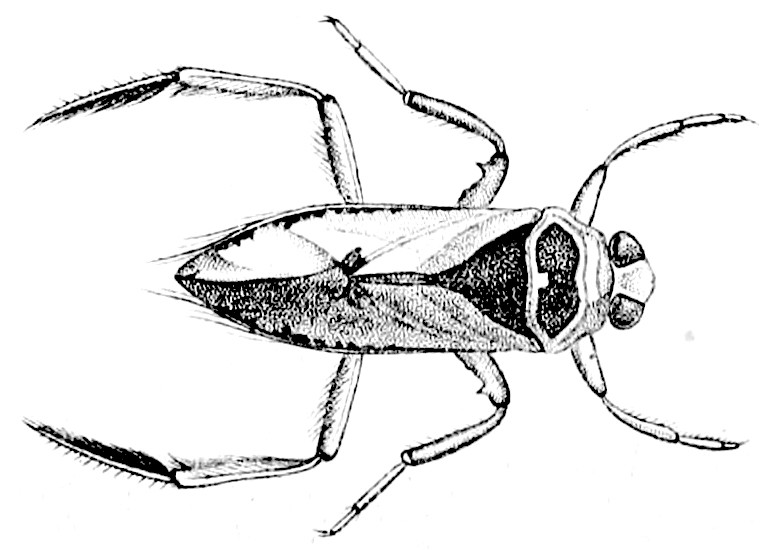
\includegraphics[width=0.45\textwidth]{NotonectidHabitus}
 \caption{Notonectidae, dorsal habitus \citep[][Plate 7, Fig. 2]{bhl37902}}
 \label{fig:notonect1}
\end{figure}

\noindent{}These insects swim upside down. How does their morphology vary from other heteropterans, given this behavior?

\subsubsection{Nepidae (water scorpions)}
\noindent{}\textit{Diagnostic characters:} Body shape variable (Figure \ref{fig:nepid1}); antennae shorter than head; ocelli absent; tarsi each comprised of 1 tarsomere; fore legs raptorial; hind legs not oarlike, hind tarsi with claws; 2 long terminal abdominal appendages called ``airstraps''.\\

\noindent{}\textit{Natural history:} \\

\begin{figure}[ht!]
 \centering
 
\includegraphics[width=0.45\textwidth]{image14}
 \caption{Nepidae, dorsal habitus}
 \label{fig:nepid1}
\end{figure}

\subsubsection{Belostomatidae (giant water bugs)}
\noindent{}\textit{Diagnostic characters:} Body large, dorso-ventrally flattened usually over \textgreater20 mm; antennae shorter than head; ocelli absent; fore legs raptorial (Figure \ref{fig:belostom1}); hind legs flat, oar-like, hind tarsi with claws; membrane of fore wing with veins.\\

\noindent{}\textit{Natural history:} \\

\begin{figure}[ht!]
 \centering
 
\includegraphics[width=0.5\textwidth]{image14}
 \caption{Belostomatidae, dorsal habitus}
 \label{fig:belostom1}
\end{figure}

\noindent{}Compare the airstraps of Belostomatidae to those of Nepidae; how are they different?\vspace{2cm}

\begin{figure}[ht!]
 \centering
 
\includegraphics[width=0.4\textwidth]{image14}
 \caption{Naucoridae, dorsal habitus}
 \label{fig:naucor1}
\end{figure}

\noindent{}Look closely at the tarsi and the apex of each leg on the following two families. Do you see any features that might be useful for skating on the water's surface?

\subsubsection{Gerridae (water striders)}
\noindent{}\textit{Diagnostic characters:} Body usually \textgreater5 mm; antennae longer than head; middle legs arising closer to hind legs than to front legs (Figure \ref{fig:gerrid1}); hind femur longer than abdomen.\\

\noindent{}\textit{Natural history:} \\

\begin{figure}[ht!]
 \centering
 
\includegraphics[width=0.5\textwidth]{image14}
 \caption{Gerridae, dorsal habitus}
 \label{fig:gerrid1}
\end{figure}

\subsubsection{Veliidae (ripple or riffle bugs)}
\noindent{}\textit{Diagnostic characters:} Body relatively small, 1.6--5.5 mm; antennae longer than head (Figure \ref{fig:veliid1}); mid-legs arise midway between fore and hind legs; hind femur shorter than abdomen.\\

\noindent{}\textit{Natural history:} \\

\begin{figure}[ht!]
 \centering
 
\includegraphics[width=0.4\textwidth]{image14}
 \caption{Veliidae, dorsal habitus}
 \label{fig:veliid1}
\end{figure}

\subsubsection{Saldidae (shore bugs)}
\noindent{}\textit{Diagnostic characters:} dorso-ventrally flattened, typically brownish; antenna with 4 antennomeres; labium with 3 sclerites; tarsus with 3 tarsomeres; membrane of fore wing with 4--5 long closed cells (Figure \ref{fig:saldid1}--\ref{fig:saldidwing}).\\

\noindent{}\textit{Natural history:} \\

\begin{figure}[ht!]
 \centering
 \begin{subfigure}[ht!]{0.27\textwidth}
  
\includegraphics[width=\textwidth]{image14}
  \caption{Dorsal habitus}
  \label{fig:saldid1}
 \end{subfigure}
 ~ %add desired spacing between images, e. g. ~, \quad, \qquad, \hfill etc. 
  %(or a blank line to force the subfigure onto a new line)
 \begin{subfigure}[ht!]{0.55\textwidth}
  
\includegraphics[width=\textwidth]{image14}
  \caption{Fore wing}
  \label{fig:saldidwing}
 \end{subfigure}
 \caption{Saldidae}\label{fig:saldid}
\end{figure}

\subsubsection{Miridae (plant bugs)}
\noindent{}\textit{Diagnostic characters:} Antenna with 4 antennomeres (Figure \ref{fig:mirid1}); ocelli absent; labium with 4 sclerites; tarsus with 3 tarsomeres; cuneus present (compare to taxon with cuneus absent, like Nabidae); membrane with 2 closed cells (Figure \ref{fig:miridwing}); wings wide, abdomen at most slightly exposed laterally.\\

\noindent{}\textit{Natural history:} \\

\begin{figure}[ht!]
 \centering
 \begin{subfigure}[ht!]{0.45\textwidth}
  
\includegraphics[width=\textwidth]{image14}
  \caption{Dorsal habitus}
  \label{fig:mirid1}
 \end{subfigure}
 ~ %add desired spacing between images, e. g. ~, \quad, \qquad, \hfill etc. 
  %(or a blank line to force the subfigure onto a new line)
 \begin{subfigure}[ht!]{0.45\textwidth}
  
\includegraphics[width=\textwidth]{image14}
  \caption{Fore wing}
  \label{fig:miridwing}
 \end{subfigure}
 \caption{Miridae}\label{fig:miridae}
\end{figure}

\subsubsection{Anthocoridae (minute pirate bugs)}
\noindent{}\textit{Diagnostic characters:} Antenna with 4 antennomeres; labium with 3 sclerites; ocelli present; tarsus with 2--3 tarsomeres; front legs not raptorial; cuneus present; membrane with no closed cells, with one or two usually rudimentary longitudinal veins (Figure \ref{fig:anthocoridwing}); wings wide, abdomen at most slightly exposed laterally (Figure \ref{fig:anthocorid1}).\\

\noindent{}\textit{Natural history:} \\

\begin{figure}[ht!]
 \centering
 \begin{subfigure}[ht!]{0.45\textwidth}
  
\includegraphics[width=\textwidth]{image14}
  \caption{Dorsal habitus}
  \label{fig:anthocorid1}
 \end{subfigure}
 ~ %add desired spacing between images, e. g. ~, \quad, \qquad, \hfill etc. 
  %(or a blank line to force the subfigure onto a new line)
 \begin{subfigure}[ht!]{0.45\textwidth}
  
\includegraphics[width=\textwidth]{image14}
  \caption{Fore wing}
  \label{fig:anthocoridwing}
 \end{subfigure}
 \caption{Anthocoridae}\label{fig:anthocorid}
\end{figure}

\subsubsection{Tingidae (lace bugs)}
\noindent{}\textit{Diagnostic characters:} body and wings with reticulate ``lace-like'' sculpture (Figure \ref{fig:tingid1}); antenna with 4 antennomeres; ocelli present; labium with 4 sclerites;  each leg with 1--2 tarsomeres; cuneus absent; membrane venation obscured by reticulate sculpture; pronotum extends posteriorly obscuring mesoscutellum.\\

\noindent{}\textit{Natural history:} \\

\noindent{}What do you think is the function of the elaborate integumental sculpturing of these bugs?\vspace{3cm}

\begin{figure}[ht!]
 \centering
 
\includegraphics[width=0.45\textwidth]{image14}
 \caption{Tingidae, dorsal habitus}
 \label{fig:tingid1}
\end{figure}

\subsubsection{Nabidae (damsel bugs)}
\noindent{}\textit{Diagnostic characters:} Antenna with 4 antennomeres; labium with 4 sclerites; ocelli present; each leg with 2--3 tarsomeres; fore leg raptorial; cuneus absent; membrane with numerous closed cells or absent; wings wide, abdomen at most slightly exposed laterally.\\

\noindent{}\textit{Natural history:} \\

\begin{figure}[ht!]
 \centering
 \begin{subfigure}[ht!]{0.4\textwidth}
  
\includegraphics[width=\textwidth]{image14}
  \caption{Lateral habitus}
  \label{fig:nabid1}
 \end{subfigure}
 ~ %add desired spacing between images, e. g. ~, \quad, \qquad, \hfill etc. 
  %(or a blank line to force the subfigure onto a new line)
 \begin{subfigure}[ht!]{0.5\textwidth}
  
\includegraphics[width=\textwidth]{image14}
  \caption{Fore wing}
  \label{fig:nabidwing}
 \end{subfigure}
 \caption{Nabidae}\label{fig:nabidae}
\end{figure}

\subsubsection{Berytidae (stilt bugs)}
\noindent{}\textit{Diagnostic characters:} antenna with 4 antennomeres; apical antennomere spindle-shaped; labium with 4 sclerites; each leg with 3 tarsomeres; fore leg not raptorial; cuneus absent; membrane with no closed cells (usually with 5 longitudinal veins); wings wide, abdomen at most slightly exposed laterally.\\

\noindent{}\textit{Natural history:} \\

\begin{figure}[ht!]
 \centering
 \includegraphics[width=0.55\textwidth]{image14}
 \caption{Berytidae, dorsal habitus}
 \label{fig:berytid1}
\end{figure}

\noindent{}\textit{Natural history:} \\

\subsubsection{Lygaeidae (seed bugs)}
\noindent{}\textit{Diagnostic characters:} Head narrower than pronotum; antenna with 4 antennomeres; labium with 4 sclerites; each leg with 3 tarsomeres; fore leg not raptorial; cuneus absent; membrane with no closed cells; wings wide, abdomen at most slightly exposed laterally; abdominal spiracles 5--7 dorsally located.\\

\noindent{}\textit{Natural history:} \\

\begin{figure}[ht!]
 \centering
 \includegraphics[width=0.55\textwidth]{image14}
 \caption{Lygaeidae fore wing}
 \label{fig:lygaeid1}
\end{figure}

\subsubsection{Geocoridae (big-eyed bugs)}
\noindent{}\textit{Diagnostic characters:} Head wider than pronotum (Figure \ref{fig:geocorid1}); antenna with 4 antennomeres; labium with 4 sclerites; ocelli present; each leg with 3 tarsomeres; fore leg not raptorial; cuneus absent; wings wide, abdomen at most slightly exposed laterally; abdominal spiracles 5--7 ventrally located.\\

\noindent{}\textit{Natural history:} \\

\begin{figure}[ht!]
 \centering
 \includegraphics[width=0.55\textwidth]{image14}
 \caption{Geocoridae habitus}
 \label{fig:geocorid1}
\end{figure}

\noindent{}Take a look at the head shape and compare to the previous few families. Do you see any differences? What might these insects feed on?\vspace{3cm}

\subsubsection{Coreidae (leaf-footed bugs)}
\noindent{}\textit{Diagnostic characters:} Head narrower and shorter than pronotum; antenna with 4 antennomeres; labium with 4 labial sclerites; ocelli present; each leg with 3 tarsomeres; cuneus absent; wings wide, abdomen at most slightly exposed laterally; hind tibia usually widened, leaf-shaped.\\

\noindent{}\textit{Natural history:} \\

\begin{figure}[ht!]
 \centering
 \begin{subfigure}[ht!]{0.35\textwidth}
  \includegraphics[width=\textwidth]{image14}
  \caption{Dorsal habitus}
  \label{fig:coreid1}
 \end{subfigure}
 ~ %add desired spacing between images, e. g. ~, \quad, \qquad, \hfill etc. 
  %(or a blank line to force the subfigure onto a new line)
 \begin{subfigure}[ht!]{0.55\textwidth}
  \includegraphics[width=\textwidth]{image14}
  \caption{Fore wing}
  \label{fig:coreidwing}
 \end{subfigure}
 \caption{Coreidae}\label{fig:coreidae}
\end{figure}

\subsubsection{Rhopalidae (boxelder bugs)}
\noindent{}\textit{Diagnostic characters:} Head narrower and shorter than pronotum; antenna with 4 antennomeres; labium with 4 sclerites; ocelli present; fore leg not raptorial; each leg with 3 tarsomeres; tibia without large, semierect spines; hind tibia usually widened, leaf-shaped; cuneus absent; scent gland absent; wings wide, abdomen at most slightly exposed laterally.\\

\noindent{}\textit{Natural history:} \\

\noindent{}This coreid looking taxon is not illustrated here. Could you find its diagnostic character the glycerine stored specimen?\vspace{3cm}

\subsubsection{Aradidae (flat bugs)}
\noindent{}\textit{Diagnostic characters:} Antenna with 4 antennomeres; number of labial sclerites: 4; ocelli absent; number of tarsomeres: 2; cuneus absent; fore leg not raptorial; wings wide, abdomen at most slightly exposed laterally ; hind tibia usually widened, leaf-shaped; head narrower and shorter than pronotum.\\

\noindent{}\textit{Natural history:} \\

\begin{figure}[ht!]
 \centering
 \includegraphics[width=0.5\textwidth]{image14}
 \caption{Aradidae habitus}
 \label{fig:aradid1}
\end{figure}

\noindent{}Given their common name and their body shape, where do you think these live?\vspace{3cm}

\subsubsection{Alydidae (broad-headed bugs)}
\noindent{}\textit{Diagnostic characters:} Antenna with 4 antennomeres; labium with 4 sclerites; ocelli present; each leg with 3 tarsomeres; head as wide and long as pronotum; cuneus absent; fore leg not raptorial; wings wide, abdomen at most slightly exposed laterally; hind tibiae not widened and leaf-shaped.\\

\noindent{}\textit{Natural history:} \\

\begin{figure}[ht!]
 \centering
 \includegraphics[width=0.45\textwidth]{image14}
 \caption{Alydidae habitus}
 \label{fig:alydid1}
\end{figure}

\subsubsection{Reduviidae (assassin and ambush bugs)}
\noindent{}\textit{Diagnostic characters:} Antenna with 4 antennomeres; ocelli present or absent; labium with 3 sclerites; each leg with 1--3 tarsomeres; cuneus absent; fore leg raptorial; prothorax usually with a ventral, longitudinal scrobe accommodating the long and robust mouthparts; wings wide, abdomen at most slightly exposed laterally.\\

\noindent{}\textit{Natural history:} \\

\begin{figure}[ht!]
 \centering
 \includegraphics[width=0.4\textwidth]{image14}
 \caption{Reduviidae habitus}
 \label{fig:reduviid1}
\end{figure}

\subsubsection{Cimicidae (bed bugs, bat bugs)}
\noindent{}\textit{Diagnostic characters:} Antenna with 4 antennomeres; labium with 3 sclerites; ocelli absent; number of tarsomeres: 2--3; wings absent.\\

\noindent{}\textit{Natural history:} \\

\begin{figure}[ht!]
 \centering
 \includegraphics[width=0.5\textwidth]{image14}
 \caption{Cimicidae habitus}
 \label{fig:cimicid1}
\end{figure}

\subsubsection{Scutelleridae (shield bugs)}
\noindent{}\textit{Diagnostic characters:} Antenna with 5 antennomeres; labium with 4 sclerites; each leg with 3 tarsomeres; cuneus absent; mesoscutellum extends posteriorly, obscuring most of abdomen (Figure \ref{fig:scutellerid1}); wings wide, abdomen at most slightly exposed laterally.\\

\noindent{}\textit{Natural history:} \\

\begin{figure}[ht!]
 \centering
\begin{subfigure}[ht!]{0.35\textwidth}
 \includegraphics[width=\textwidth]{image14}
 \caption{Scutelleridae habitus}
 \label{fig:scutellerid1}
\end{subfigure}
 \qquad %add desired spacing between images, e. g. ~, \quad, \qquad, \hfill etc. 
  %(or a blank line to force the subfigure onto a new line)
\begin{subfigure}[ht!]{0.35\textwidth}
 \includegraphics[width=\textwidth]{image14}
 \caption{Pentatomidae habitus}
 \label{fig:pentatomid1}
\end{subfigure}
 \caption{}\label{fig:pentscut}
\end{figure}

\subsubsection{Pentatomidae (stink bugs)}
\noindent{}\textit{Diagnostic characters:} antenna with 5 antennomeres (Figure \ref{fig:pentatomid1}); labium with 4 sclerites; each leg with 3 tarsomeres; cuneus absent; mesoscutellum extends posteriorly but does not obscure most of abdomen; fore leg not raptorial; wings wide, abdomen at most slightly exposed laterally.\\

\noindent{}\textit{Natural history:} \\

\FloatBarrier

\section*{Acknowledgments}
Andrew R. Deans and Istv\'an Mik\'o wrote the text. Many of the illustrations were generously made available by the Biodiversity Heritage Library (\url{http://biodiversitylibrary.org}) and the photographers at Flickr (\url{http://flickr.com}).

\FloatBarrier
% adding bibliography here
\bibliographystyle{apalike}
\bibliography{bib}

\end{document}

\subsubsection{Cydnidae (burrowing bugs)}
\noindent{}\textit{Diagnostic characters:} Pennsylvania species always brown to black; antenna with 5 antennomeres; 4 labial sclerites present; fore leg not raptorial, but legs spiny; tibia with large, semierect spines; each leg with 3 tarsomeres (Figure \ref{fig:cydnid1}); cuneus absent; mesoscutellum extends posteriorly but does not obscure much of the abdomen; wings wide, abdomen at most slightly exposed laterally.\\

\noindent{}\textit{Natural history:} \\

\begin{figure}[ht!]
 \centering
 \includegraphics[width=0.35\textwidth]{image09}
 \caption{Cydnidae habitus}
 \label{fig:cydnid1}
\end{figure}

\subsubsection{Naucoridae (creeping water bugs)}
\noindent{}\textit{Diagnostic characters:} antennae shorter than head; ocelli absent; hind legs not oar-like, hind tarsi with claws; fore legs raptorial (Figure \ref{fig:naucor1}); membrane of fore wing without veins; look like shorter, smaller Belostomatidae.\\

\noindent{}\textit{Natural history:} \\


\subsubsection{Issidae}
\noindent{}\textit{Diagnostic characters:} antennae arise below eyes (Figure \ref{fig:issid1}); median, emarginated area of the head present ; fork-like vein present on fore wing anal region; fore wings without many costal crossveins (compare to Flatidae); fore wings often as long as or shorter than abdomen ; hind tibiae with 1 or 2 robust lateral and numerous apical spines (Figure \ref{fig:issid2}).\\

\begin{figure}[ht!]
 \centering
 \begin{subfigure}[ht!]{0.45\textwidth}
  \includegraphics[width=\textwidth]{image05}
  \caption{Habitus}
  \label{fig:issid1}
 \end{subfigure}
 ~ %add desired spacing between images, e. g. ~, \quad, \qquad, \hfill etc. 
  %(or a blank line to force the subfigure onto a new line)
 \begin{subfigure}[ht!]{0.35\textwidth}
  \includegraphics[width=\textwidth]{image35}
  \caption{Hind legs}
  \label{fig:issid2}
 \end{subfigure}
 \caption{Issidae}\label{fig:issid}
\end{figure}


\subsubsection{Flatidae (wedge leafhoppers)}
\noindent{}\textit{Diagnostic characters:} antennae arise below eyes on sides of head (Figure \ref{fig:flatid2}); median, emarginated area of the head present ; fork-like vein present on fore wing anal region; fore wings with many costal crossveins (Figure \ref{fig:flatid1}); body wedge-shaped, flattened from side to side, wings broad, triangular.\\

\noindent{}\textit{Natural history:} \\

\begin{figure}[ht!]
 \centering
 \begin{subfigure}[ht!]{0.45\textwidth}
  \includegraphics[width=\textwidth]{image29}
  \caption{Habitus}
  \label{fig:flatid1}
 \end{subfigure}
 ~ %add desired spacing between images, e. g. ~, \quad, \qquad, \hfill etc. 
  %(or a blank line to force the subfigure onto a new line)
 \begin{subfigure}[ht!]{0.35\textwidth}
  \includegraphics[width=\textwidth]{image33}
  \caption{Anterior view of head}
  \label{fig:flatid2}
 \end{subfigure}
 \caption{Flatidae}\label{fig:flatid}
\end{figure}